%%%%%%%%%%%%%%%%%%%%%%%%%%%%%%%%%%%%%%%%%%%%%%%%%%%%%%%%%%%%%%%%%
%%%%%%%%%%%%%%%%%%%%%%%%%%%%%%%%%%%%%%%%%%%%%%%%%%%%%%%%%%%%%%%%%
\chapter{PK Macros}
\label{sec:PKMacros}

%%%%%%%%%%%%%%%%%%%%%%%%%%%%%%%%%%%%%%%%%%%%%%%%%%%%%%%%%%%%%%%%%
\section{Introduction}
A long standing problem in Pharmacometrics is how to define effectively PK models, 
without using ODEs, in a tool-independent way. There are many tool-specific solutions, 
each of them using their own ways to define PK models. 
After a thorough analysis of a number of available approaches, the MLXTRAN PK macro 
system has been selected to be supported in PharmML 
\cite{MLXTRANforMonolix:2014}.  It has the following features 
\begin{itemize}
\item
Tool-independent, but easily translatable to tool-specific libraries
\item
User friendly and easy to learn for users new to the field
\item
Flexible and providing consistent specification of compartmental PK models
\item
More models can be specified without ODEs, compared to nmadvan/PREDPP
\item
No limitations will be imposed, compared to nmadvan/PREDPP:
\begin{itemize}
\item
All PREDPP library models with underlying analytical solutions (ADVAN1-4, 11-12) can be specified. 
Templates are provided for these to help NONMEM users, see Section \ref{subsec:PREDPPinMACROS}.
\item
The PREDPP library models applying matrix exponential-based solutions (ADVAN 5, 7) are already 
being defined in a way very similar to the macro-based solution proposed.
\item
The PREDPP library models applying numerical ODE solution (ADVAN 6, 8-9, 10, 13) can still be 
specified by using ODEs explicitly (or by using/mixing with macro-definitions).
\end{itemize}
\end{itemize}

Adopting the PK macros should allow seamless translation of models between MDL and 
PharmML and MLXTRAN. Therefore, in the PharmML implementation of the macros we tried 
to stay as close as possible to the original MLXTRAN specification. We had to make sure 
that the macros, their attributes and possible assignments are defined in a unambiguous 
way. In the sections \ref{subsec:encodingRules} and \ref{subsec:fixedArguments} we 
explain the rules to be followed in their implementation and the translation process to and 
from PharmML.


%%%%%%%%%%%%%%%%%%%%%%%%%%%%%%%%%%%%%%%%%%%%%%%%%%%%%%%%%%%%%%%%%%%%%%
\subsection{The macro idea}
Figure \ref{fig:flowDiagram} visualises the principle of the PK macros solution and its use. The module 
within the inner MDL/PharmML box shows few example PK macros and their attributes using which a 
PK model can be formulated. 
\begin{figure}[htb!]
\centering
  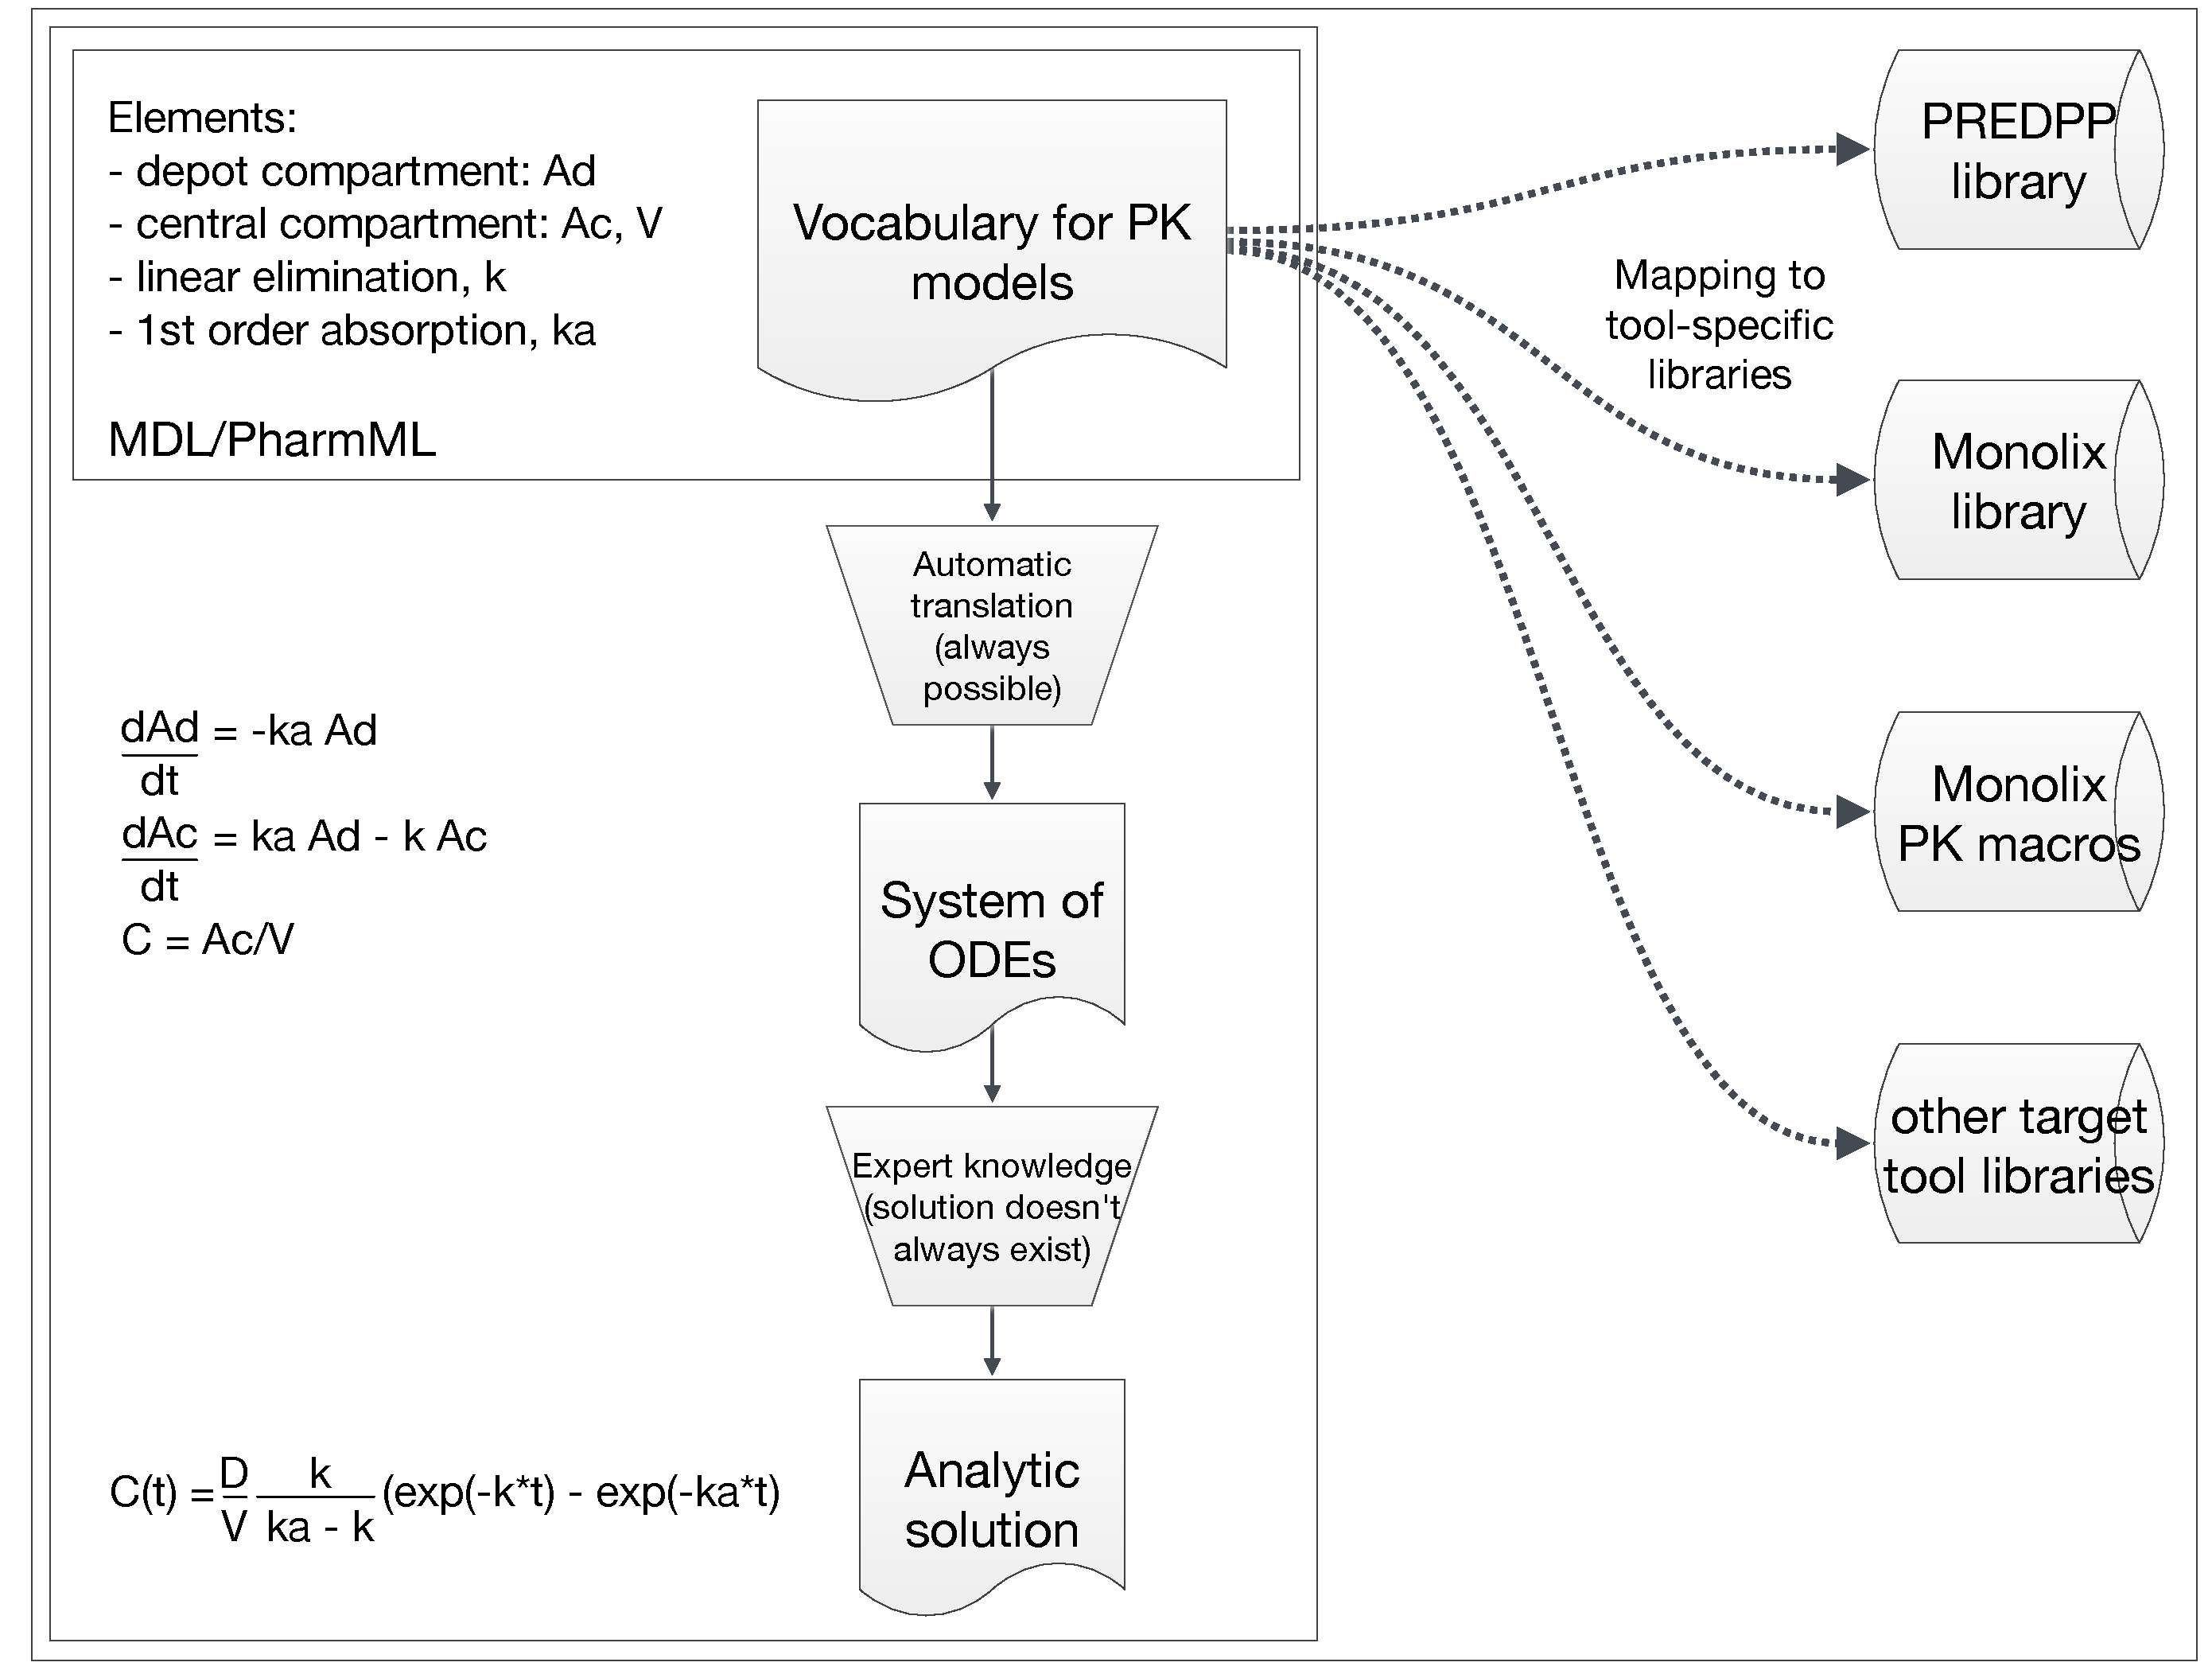
\includegraphics[width=160mm]{pics/PKmacrosPrinciple.pdf}
 \caption{A diagram explaining how the PK macro system can be used in practise. The inner 
 MDL/PharmML box contains the information to be stored in PharmML, i.e. the macros and arguments 
 from the PK model vocabulary. It can then be automatically translated into a set of ODEs and for some 
 models there exists an analytic solution. Models encoded using the controlled vocabulary can be 
 mapped to tool specific implementations (dotted lines).}
 \label{fig:flowDiagram}
\end{figure}
In this case four macros, with one or more arguments, are used to encode a basic \emph{oral 1-compartment 
model with linear elimination} consisting of the following items
\begin{enumerate}
\item
depot compartment, with amount \emph{Ad},
\item
central compartment, with amount \emph{Ac} and volume \emph{V},
\item
oral administration, 1$^{st}$ order absorption with rate constant \emph{ka}, and 
\item
linear elimination, with rate constant \emph{k}.
\end{enumerate}
%For other examples see Tab.\ref{tab:MappingTable}. 
This is the \emph{only} information that needs to be encoded in PharmML for this particular PK model. It 
corresponds to the following macro
\lstset{language=NONMEMdataSet}
\begin{lstlisting}
		compartment(cmt=1,concentration=Cc,volume=V) 
		oral(cmt=1, ka) 
		elimination(cmt=1, k)
\end{lstlisting}
Any information about input, i.e. dosing times and amounts will be stored in the dataset 
or explicitly within the \xelem{TrialDesign}.

The key \marginpar{\HandCuffLeft} realisation is that every set of such macro statements, 
if correctly defined, can be translated automatically into a unique set of ODE's and/or 
algebraic equations, in this case:
\begin{align}
\frac{dAd}{dt} &= -ka \times Ad \nonumber \\
\frac{dAc}{dt} &= ka \times Ad - k \times Ac  \nonumber \\
C &= Ac/V \nonumber
\end{align}

Moreover, for some models such as the above one, there exists an analytic solution. This however cannot 
be derived automatically for an arbitrary ODE system. It requires a powerful symbolic calculation 
software or expert knowledge. Once the PK model macros and their attribute set have been defined, 
a mapping to tool-specific libraries can be provided, see Fig.\ref{fig:flowDiagram}. 
This again requires expert knowledge of each particular tool. 



%%%%%%%%%%%%%%%%%%%%%%%%%%%%%%%%%%%%%%%%%%%%%%%%%%%%%%%%%%%%%%%%%%%%%%%
\section{PK macros in PharmML}
\label{subsec:PKmacros}

\subsection{MLXTRAN macros}
\label{sec:MLXTRANmacros}

PK macros offer an equation-free encoding solution for pharmacokinetic models. 
The novel system allows to implement in MLXTRAN virtually any compartmental 
model within well-defined constraints. See \cite{MLXTRANforMonolix:2014} for a detailed 
description. The following table lists the available PK macros with their arguments. 

\begin{table}[ht!]
\centering
\begin{tabular}{lll}
  \hline
  \hline
Component & Macro & Arguments \\
  \hline
Compartment 			& \textit{compartment}	 	& cmt, amount, volume, concentration \\
Peripheral compartment	& \textit{peripheral}			& \textbf{kij}, \textbf{k$\_$i$\_$j}, amount, volume, concentration \\
Effect compartment 		& \textit{effect} 				& cmt, \textbf{ke0}, concentration \\
Absorption from a depot 	& \textit{depot} 				& type/adm, \textbf{Tlag}, \textbf{p}, target, \textbf{Tk0}, \textbf{ka}, \textbf{Ktr}/\textbf{Mtt} \\
Absorption for IV dose 	& \textit{iv} 				& cmt, type/adm, \textbf{Tlag}, \textbf{p} \\
0-order absorption 		& \textit{absorption}			& cmt, type/adm, \textbf{Tlag}, \textbf{p}, \textbf{Tk0} \\[-.5ex]
					& or \textit{oral}				& \\
1st order absorption 	& \textit{absorption}			& cmt, type/adm, \textbf{Tlag}, \textbf{p}, \textbf{ka}, \textbf{Ktr}/\textbf{Mtt} \\[-.5ex]
					& or \textit{oral}				& \\
Linear elimination 		& \textit{elimination}			& cmt, volume, \textbf{k}, \textbf{CL} \\
MM elimination 		& \textit{elimination}			& cmt, \textbf{Km}, \textbf{Vm} \\
Transfer 				& \textit{transfer}			& from, to, \textbf{kt} \\
  \hline
\end{tabular}
\caption{PK macros and their arguments as used in MLXTRAN, based on 
\cite{MLXTRANforMonolix:2014}. Note that there are more components listed, 
10, than macros, 9, actually defined in the MLXTRAN system. Different absorption 
and elimination types are listed separately for better readability. The arguments can be 
devided in two groups. Those who can act alone in the macro are marked with bold font,
all others need to be assigned a numerical value or a symbol reference, see explanation in text.}
\label{tab:MLXPLORElibrary}
\end{table}
One can distinguish two types of arguments, see Table \ref{tab:MLXPLORElibrary}. 
The arguments marked with \textbf{bold} font, can be simply references to identifiers 
defined somewhere else in the model file such as \emph{ka} or \emph{Tlag}. The remaining 
arguments cannot be left unassigned and have to be explicitly specified as attributes 
of the \xelem{Value} element and subsequently assigned a numerical value or 
symbol reference, e.g. \emph{cmt} or \emph{amount}. See Section 
\ref{subsec:encodingRules} for the detailed explanation.

%An essential aspect of the macros is their connectivity to the 
%remaining model elements and the data. The necessary extensions in the current structure are
%discussed, for the input in section \ref{subsec:LinkingMacrosDatasets} and for the output in 
%section \ref{subsec:macroOutputLink}. 

%{\color{red} \scshape{NEW}}
%%%%%%%%%%%%%%%%%%%%%%%%%%%%%%%%%%%%%%%%%%%%%%%%%%%%%%%%%
\subsection{Encoding rules}
\label{subsec:encodingRules}
To provide the full support for MLXTRAN PK macros, all macros and their (unordered) named 
arguments have to be encodable, see Table \ref{tab:MLXPLORElibrary}. Every macro has its own 
PharmML element, e.g. the basic \emph{concentration} macro with all its arguments, encoded as \xelem{Value} 
elements, will be encoded within the \xelem{Concentration} element. The optional attribute \xatt{argument}
is assigned a value corresponding to the argument of the macro. 

%\subparagraph{The basic principle for the implementation and translation to and from PharmML} 
%Macros arguments are encoded as attributes of macro elements only if an assignment is required, 
%otherwise we just refer to them with the standard \xelem{SymbRef} element. 

As mentioned above, there are two types of arguments, and the following rules 
are defined to achieve a consistent macro definition and its interpretation:
\begin{itemize}
\item
\textbf{bold} arguments (\emph{can act alone}) can be references to symbol identifiers defined in other 
places in the model, such as \xatt{k}, \xatt{ka} etc.
\begin{itemize}
\item
cannot be assigned numerical values or expressions within the macro -- 
all such assignments must be defined outside the \xelem{PKmacros} element, for example in the 
\xelem{ParameterModel} or in the \xelem{ModellingSteps} section
\item
if an argument, e.g. 'k', is specified in a macro only, as shown below
\lstset{language=NONMEMdataSet}
\begin{lstlisting}
		elimination(cmt=1, k)
\end{lstlisting}
then a simple \xatt{SymbIdRef} is sufficient
 \lstset{language=XML}
\begin{lstlisting}
                <Elimination>
                    <!-- cmt argument omitted -->
                    <Value>
                        <ct:SymbRef blkIdRef="pm1" symbIdRef="k"/>
                    </Value>
                </Elimination>
\end{lstlisting}
but it must be defined in a parameter model, here \xatt{pm1}.
\item
if a symbol identifier, here 'k1', is assigned to the key-word argument \xatt{k}, e.g.
\lstset{language=NONMEMdataSet}
\begin{lstlisting}
		elimination(cmt=1, k=k1)
\end{lstlisting}
 then both the keyword as argument, \xatt{k}, and the \xatt{symbIdRef}, \xatt{k1} are required 
 \lstset{language=XML}
\begin{lstlisting}
                <Elimination>
                    <!-- cmt argument omitted -->
                    <Value argument="k">
                        <ct:SymbRef blkIdRef="pm1" symbIdRef="k1"/>
                    </Value>
                </Elimination>
\end{lstlisting}
\end{itemize}
\item
all \textit{other} arguments (which \emph{cannot act alone}), e.g. 'cmt' or 'amount' as in the following macro
\lstset{language=NONMEMdataSet}
\begin{lstlisting}
		compartment(cmt=1, amount=Ac)
\end{lstlisting}
 \lstset{language=XML}
have to be specified as attributes first and subsequently assigned a numerical value 
or a symbol reference using element \xatt{SymbRef} as in the following code snippet
\begin{lstlisting}
                <Compartment>
                    <Value argument="cmt">
                        <ct:Int>1</ct:Int>
                    </Value>
                    <Value argument="amount">
                        <ct:SymbRef symbIdRef="Ac"/>
                    </Value>
                </Compartment>
\end{lstlisting}
\end{itemize}


%For example, the \emph{elimination} macro defining the linear elimination with rate constant \xatt{k}
%from the first compartment reads
%\lstset{language=NONMEMdataSet}
%\begin{lstlisting}
%		elimination(cmt=1, k)
%		OR
%		elimination(cmt=1, k=k1)		
%		NOT ALLOWED
%		elimination(cmt=1, k = 0.5)		
%\end{lstlisting}
%and is encoded in PharmML as
%\lstset{language=XML}
%\begin{lstlisting}
%            <!-- omitted other model elements-->
%                <Elimination>
%                    <Value argument="cmt">
%                        <ct:Int>1</ct:Int>
%                    </Value>
%                    <Value>
%                        <ct:SymbRef blkIdRef="pm1" symbIdRef="k"/>
%                    </Value>
%                    OR
%                    <Value argument="k">
%                        <ct:SymbRef blkIdRef="pm1" symbIdRef="k1"/>
%                    </Value>
%                </Elimination>
%            </PKmacros>
%        </StructuralModel>
%\end{lstlisting}
%This code makes the above principle and these two implementation options clear. In the first case, 
%an assignment is necessary. The attribute \xatt{argument="cmt"} is used to specify the compartment argument 
%of the macro \xelem{Elimination} and in the next line the number '1' is assigned to it.
%
%In the second case, the elimination rate parameter \xatt{k} is simply referred to without an assignment. 
%The mandatory here \xatt{blkIdRef} attribute points to the parameter model, \xatt{pm1}, where \xatt{k} 
%is expected to be defined.


%%%%%%%%%%%%%%%%%%%%%%%%%%%%%%%%%%%%%%%%%%%%%%%%%%%%%%%%%
\subsection{Fixed argument values and exceptions}
\label{subsec:fixedArguments}
All but one macro have a fixed set of arguments, e.g. the \xatt{compartment} can take only these predefined
four arguments: \xatt{\{cmt, amount, volume, concentration\}}. The exception is the \xatt{peripheral} macro with three fixed
arguments \xatt{\{amount, volume, concentration\}} and a variable one, \xatt{k\_ij or k\_i\_j}, where \xatt{i} and
\xatt{j} stand for input and output compartment, respectively. These compartments numbers are set 
according to the model configuration. 

For example, in the case of models ADVAN11 or 12, see section \ref{subsubsec:ADVAN12} 
for a complete description of the latter, 
we need to set the \xatt{kij} argument names accordingly to the model specification, 
meaning the macro 
\lstset{language=NONMEMdataSet}
\begin{lstlisting}
		peripheral(k12, k21, amount=Ap1)
\end{lstlisting}
will be implemented as shown in the following snippet
\lstset{language=XML}
\begin{lstlisting}
                <Peripheral>
                    <Value>
                        <ct:SymbRef blkIdRef="pm1" symbIdRef="k12"/>
                    </Value>
                    <Value>
                        <ct:SymbRef blkIdRef="pm1" symbIdRef="k21"/>
                    </Value>
                    <!-- omitted amount argument -->
                </Peripheral>
\end{lstlisting}

The \xatt{k\_ij or k\_i\_j} attributes are a special case in that an assignment in the macro 
formulated as
\lstset{language=NONMEMdataSet}
\begin{lstlisting}
		peripheral(k12, k21 = k_test, amount=Ap1)
\end{lstlisting}
will be translated to PharmML as
\lstset{language=XML}
\begin{lstlisting}
                <Peripheral>
                    <Value>
                        <ct:SymbRef blkIdRef="pm1" symbIdRef="k12"/>
                    </Value>
                    <Value argument="k21">
                        <ct:SymbRef blkIdRef="pm1" symbIdRef="k_test"/>
                    </Value>
                    <!-- omitted amount argument -->
                </Peripheral>
\end{lstlisting}
Note the difference between the implementation of the two first arguments. 
The first argument, \xatt{k12}, is implemented as before because no assignment
is required. In the second case we use the \xatt{argument} attribute to inform 
the target tool about the meaning of the assigned parameter. Therefore, the 
symbol \xatt{k12} is not a parameter itself and \xatt{k\_test} serves as the 
transfer parameter \xatt{kij} between compartment 1 and 2, which can be defined 
in the parameter model \xatt{pm1} and can be assigned any value in the 
\xelem{ModellingSteps} section.


%\newpage
%%%%%%%%%%%%%%%%%%%%%%%%%%%%%%%%%%%%%%%%%%%%%%%%%%%%%%%%%
\subsection{Macros and target tools}
\label{subsec:LinkingMacrosDatasets}

One of the main reasons to introduce the system of macros is that they offer a flexible 
and efficient way of encoding PK models. The proposed macros are fully compatible with 
Monolix and its data format, see Appendix B in \cite{Monolix4.3.2UserGuide:2014}. 

Of course, from the perspective of the interoperability platform \marginpar{\HandCuffLeft}
it is crucial that the models stored in PharmML using macros can be unambiguously translated 
to NONMEM and other target tools. Especially the compatibility with the predefined PREDPP 
routines (i.e. ADVAN 1-4 and 10-12) is essential because of their popularity among the 
NONMEM modellers community. 

To understand the required translation rules, the knowledge of relevant NONMEM and 
MONOLIX features and the dataset formats these target tools use is helpful. 
For convenience, the most essential differences between these tools/formats from the 
perspective of the macros and their usage are listed here
\begin{itemize}
\item
In PREDPP (but only when using ADVAN 1-4, 10-12 routines) the \emph{DEPOT} 
compartment is always considered as the $1^{st}$ compartment, the central compartment 
as $2^{nd}$ and the peripheral compartments as $3^{rd}$, $4^{th}$ etc. 
\item
In contrast, MONOLIX doesn't assign a number to the \emph{DEPOT} 
compartment at all and the numbering starts usually with the central compartment. 
\item
The CMT column, standard in NONMEM dataset, is not used in Monolix. It uses an ADM 
column instead.
\end{itemize}

%To provide such flexibility we have to 
%ensure that they can handle, for start, the three basic data formats 
%\begin{itemize}
%\item
%NONMEM dataset, as described in \cite{NONMEM:2009} (with restrictions such as 
%no support for PREDPP keywords and special encoding tricks)
%\item
%MONOLIX' version, a modified NONMEM dataset, see a detailed specification in \cite{Monolix4.3.2UserGuide:2014}.
%\item
%\xelem{TrialDesign} model provides the possibility to store data records in a tool-independent manner. 
%\xelem{IndividualDosing} element is the place where relevant dosing data can be encoded inline
%or be referred to from an external datafile. The actual mapping is defined within the \xelem{Activity}
%tag.  
%\end{itemize}
%There are many incompatible differences between these dataset formats, \marginpar{\HandCuffLeft} 
%here just a couple relevant points from the point of view of the PK macros


%Due to the lack of an common data format and in order to make sure that the macros can work 
%both with Monolix, NONMEM and \xelem{TrialDesing} coded datasets we needed a modification 
%in the original MLXTRAN macros.
%
%\begin{figure}[ht!]
%\centering
% 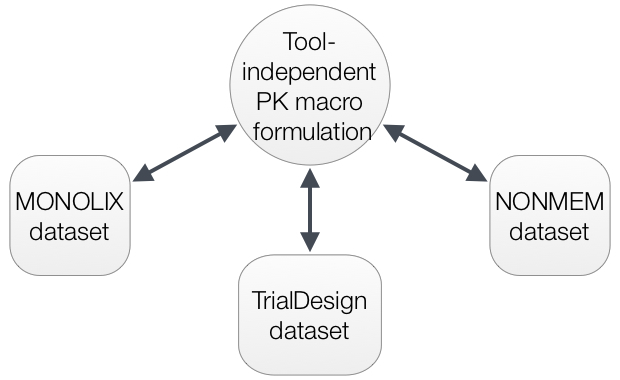
\includegraphics[width=0.6\textwidth]{pics/MacrosDatasets}
%\caption{Macros are suppose to work with Monolix, NONMEM and \xelem{TrialDesing} coded 
%datasets. }
%\label{fig:MacrosDatasets}
%\end{figure}

%\subsubsection{Modifications}
%Figure \ref{fig:ComplexModel3A} and Table \ref{tab:datasetComparison} will be used 
%to illustrate the problem. Two administrations are defined, one oral, one intravenous.
%While MONOLIX (left) doesn't assign a number to the depot compartment, 
%NONMEM (right) does. The differences are inter-connected with the format of the dataset 
%compatible with each model version. Monolix uses administration type number stored 
%in the ADM column to identify the administration process. NONMEM requires a CMT 
%column in the dataset to link a drug administration with its target. 
%
%To describe an oral administration in the original MONOLIX macro system two lines 
%of code are required and is sufficient to inform the tool about the dosing process
%\lstset{language=NONMEMdataSet}
%\begin{lstlisting}
%		compartment(cmt=1, volume=V, concentration=Cc)
%		oral(adm=1, cmt=1, ka)
%\end{lstlisting}
%
%
%However, to make the macro work with the NONMEM dataset, 
%Figure \ref{tab:datasetComparison} (RIGHT), the following modifications (in red) 
%are required
%\lstset{language=NONMEMdataSet}
%\begin{lstlisting}
%		compartment(cmt=1, volume=V, concentration=Cc)
%		[*compartment(cmt=2, amount=Depot)*]
%		oral(adm=1, [*fromCmt=2,*] cmt=1,k)
%\end{lstlisting} 
%A new \xatt{compartment} macro for the depot needs to be defined and to make 
%the connection with the target compartment work a new attribute \xatt{fromCmt}
%has to be introduced.

\subsubsection{An illustrative example}
Figure \ref{fig:ComplexModel_Rules} and datasets in Table \ref{tab:C3ModelData} 
give us some clues about two alternative interpretations for a model with at 
least one oral administration, dependent on the target tool. Note, that apart from a
few predefined models, such as ADVAN1-4 and 10-12, one can assign an arbitrary 
number to the  (first) depot compartment in the NONMEM dataset. This is exactly what 
happens in this example. While in MONOLIX we would have only two compartments 
with assigned number to them, all four compartments have numbers assigned in NONMEM,
Figure \ref{fig:ComplexModel_Rules} (right). This means that when translating a model 
from PharmML, a transformation of the associated dataset is required. 

It is therefore possible to translate a macro and dataset, utilising the ADM column to identify 
administrations, used by Monolix into an PREDPP/ADVAN based NONMEM encoding 
system with data set using the CMT column, see Figure \ref{fig:ComplexModel_Rules} and
Table \ref{tab:C3ModelData}.

\begin{figure}[h!]
\centering
 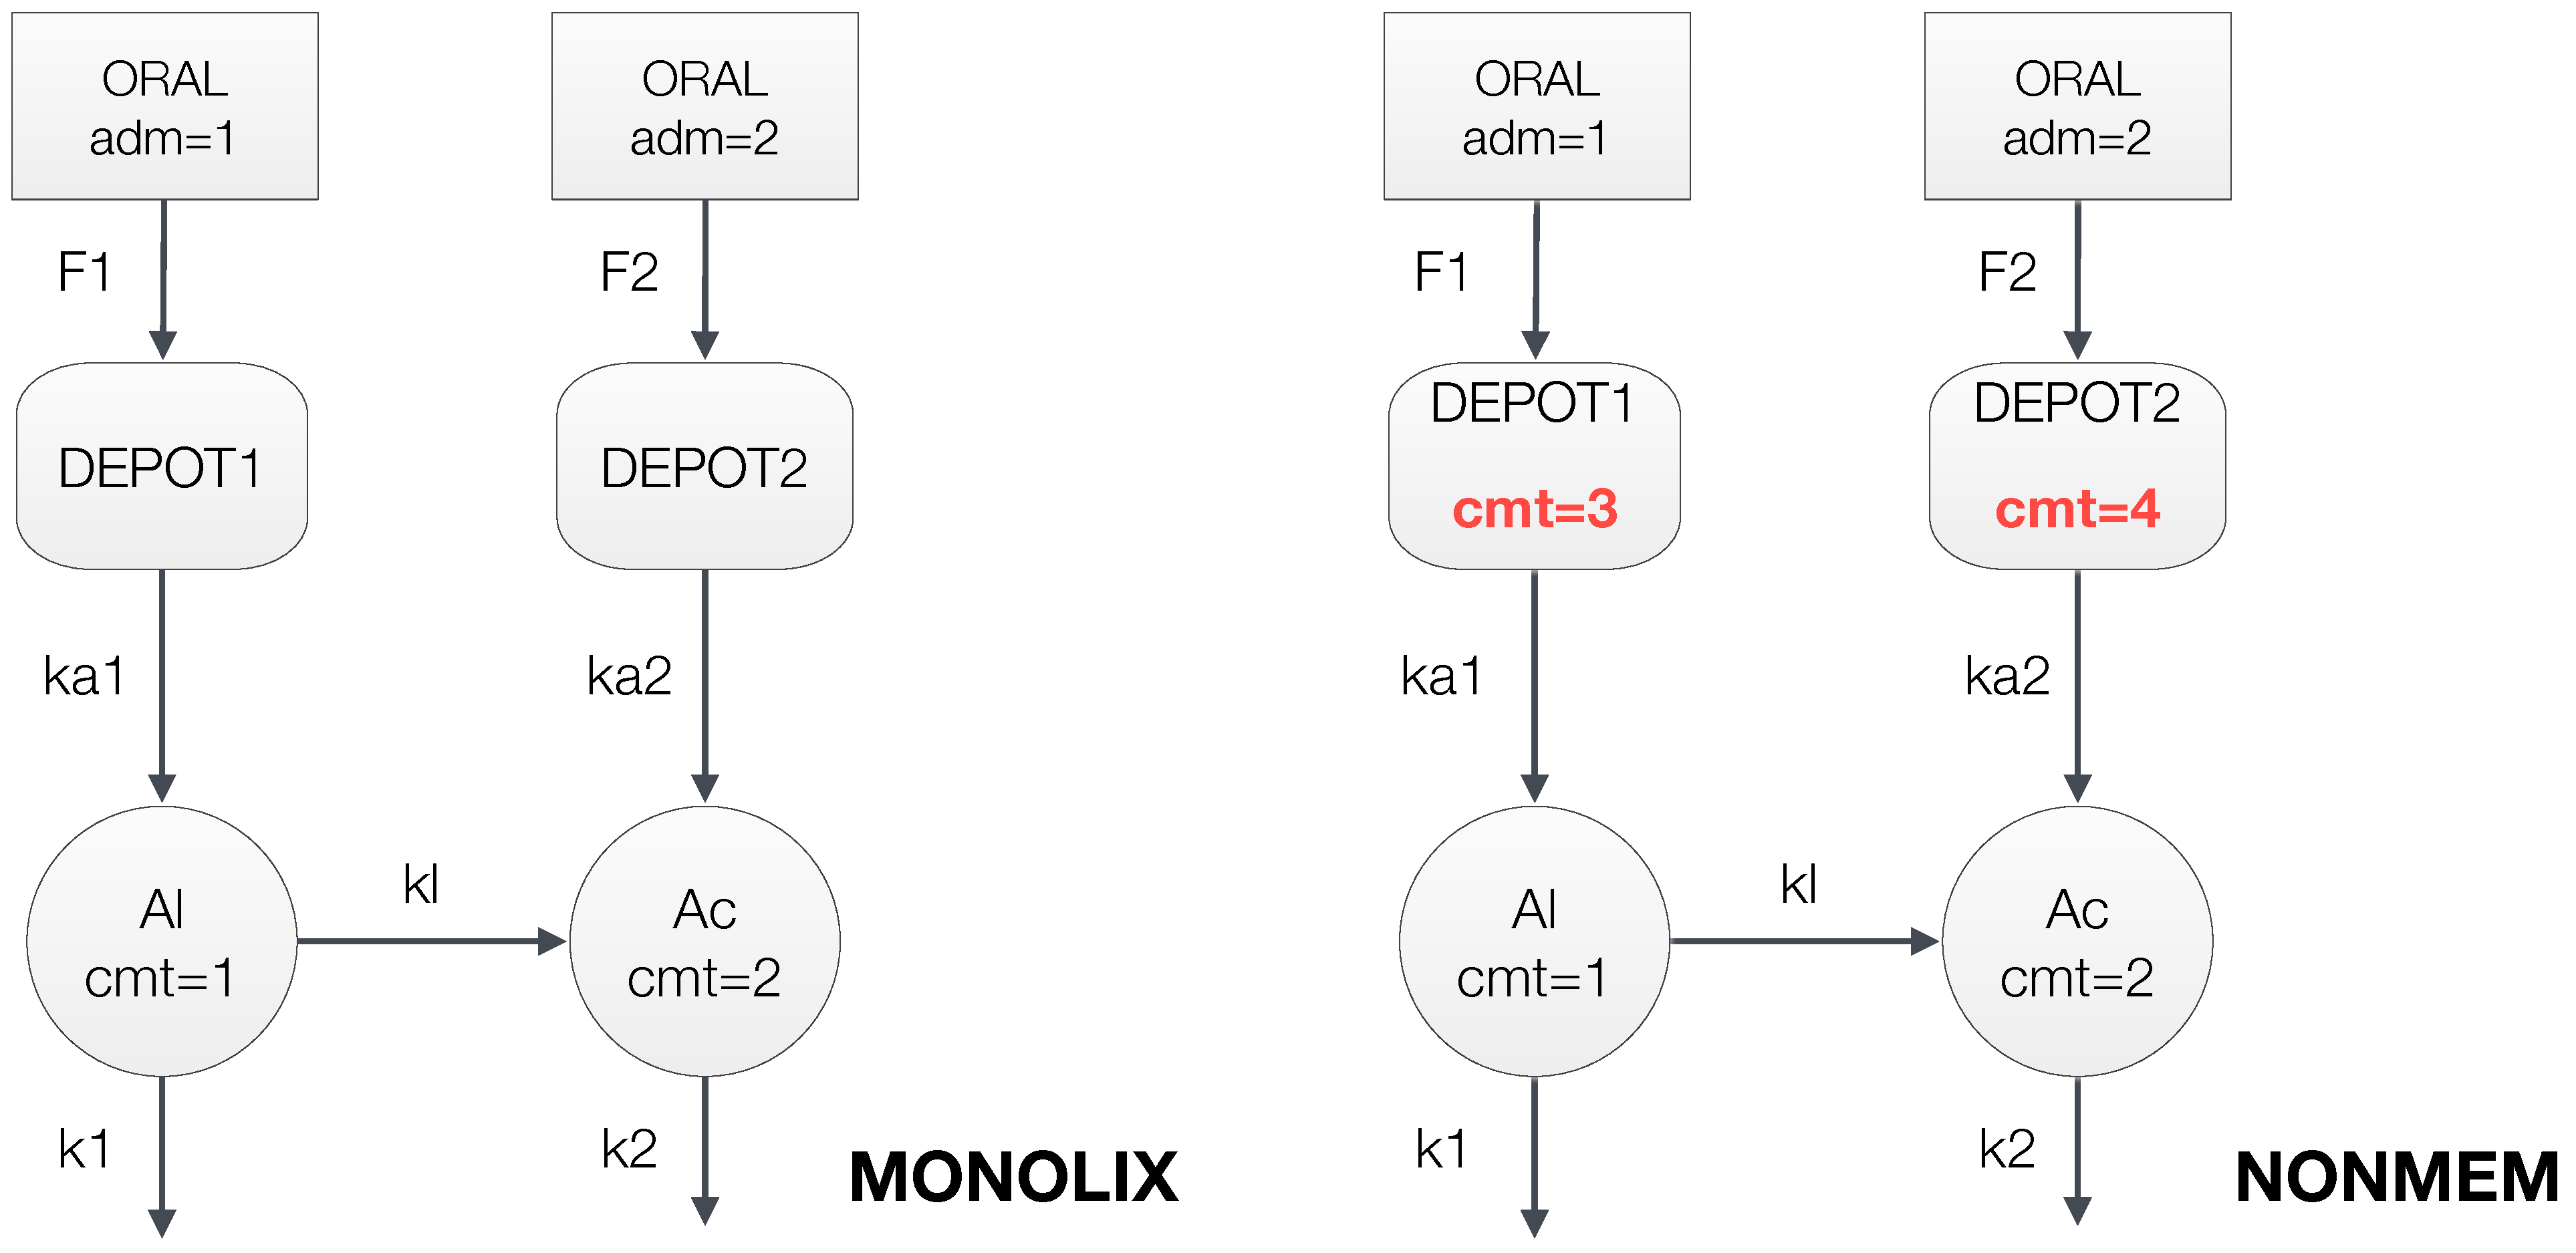
\includegraphics[width=140mm]{pics/ComplexModel_Rules.pdf}
\caption{Two interpretations for a model with two oral administrations.
While MONOLIX (left) doesn't assign a number to the depot compartments, 
NONMEM (right) does. The translation of macro coded models to target tools 
requires in this case changes in the dataset as well, see Table \ref{tab:C3ModelData}.}
\label{fig:ComplexModel_Rules}
\end{figure}

\begin{table}[h!]
\footnotesize
\parbox{.5\linewidth}{
\centering
\begin{tabular}{ccccc}
  \hline
   \multicolumn{5}{c}{\textbf{MONOLIX}} \\
  \hline
ID	& TIME  & AMT	 & \textbf{ADM}  &	Y \\
  \hline
1	& 6	    & 10	& \textbf{1}	 & . \\
1	& 9	    & 20	& \textbf{2}	 & . \\
1	& 18	    & 10	& \textbf{1}	 & . \\
1	& 33	    & 20	& \textbf{2}	 & . \\
...     &  ...     &  ...     &  ...  & ... \\
1	& 0	    & .	& .	& 0 \\
1	& 12	    & .	& .	& 1.18 \\
...     &  ...     &  ...     & ...  & ...\\
\end{tabular}
}
\hfill
\parbox{.5\linewidth}{
\centering
\begin{tabular}{ccccc}
  \hline
   \multicolumn{5}{c}{\textbf{NONMEM}} \\
  \hline
ID	& TIME  & AMT	 & \textbf{\textcolor{red}{CMT}} &	DV \\
  \hline
1	& 6	    & 10	& \textbf{\textcolor{red}{3}}	 & . \\
1	& 9	    & 20	& \textbf{\textcolor{red}{4}}	 & . \\
1	& 18	    & 10	& \textbf{\textcolor{red}{3}}	 & . \\
1	& 33	    & 20	& \textbf{\textcolor{red}{4}}	 & . \\
...     &  ...     &  ...     &  ...  & ... \\
1	& 0	    & .	& 1	& 0 \\
1	& 12	    & .	& 1	& 1.18 \\
...     &  ...     &  ...     & ...  & ...\\
\end{tabular}
}
\caption{MONOLIX and NONMEM datasets for the model above, Figure 
\ref{fig:ComplexModel_Rules}. The translator has to make sure that the numbers 
in the ADM column of the former are properly converted to the CMT column in the latter dataset.}
\label{tab:C3ModelData}
\end{table}
%See Appendix \ref{sec:PKMacrosAppendix} for more examples.

\subsubsection{Basic translation rules}
The following few basic translation rules should be treated merely as a guidance
because they do not cover the whole aspect of the model/data handling within the 
interoperability platform but are limited to the models encoded with macros. 
A more careful analysis is required to cover the structural model exchange between 
the key target tools and associated datasets.

%The flow of the data within the framework \marginpar{\HandCuffLeft}  has been so far 
%successfully avoided/neglected and needs to return to the agenda again. 

\subparagraph{A -- Models corresponding to ADVAN 1-4 and 10-12}
Fortunately, the translation of models encoded with macros and having their equivalents 
in routines ADVAN1-4 and 10-12 in PREDPP and their datasets is straightforward. 
Simply, one has to translate a corresponding macro into its equivalent ADVAN 
routine and then to rename the ADM column in the MONOLIX data set into CMT, 
see for more details and examples in Section \ref{subsec:PREDPPinMACROS}
and \ref{subsec:PREDPPinMACROSExamples}.

\subparagraph{B -- All other models}
For every oral administration one new depot compartment needs to be introduced
and assigned a number. The Figure \ref{fig:ComplexModel_Rules} and datasets 
in Table \ref{tab:C3ModelData} can again help to understand what is required. 

In this example, \xatt{adm=1} and \xatt{adm=2} denote two oral administrations. 
In the NONMEM system, Figure \ref{fig:ComplexModel_Rules} (right), '1' and '2' are  
assigned to the central and peripheral compartment respectively, as in the MONOLIX 
case, so that the next free numbers, '3' and '4', will be assigned to the depot 
compartments. 

Next, the NONMEM dataset needs to be produced based on the information stored 
in the MONOLIX dataset in such a way that it will match the new compartment 
numbering scheme with the CMT column replacing the ADM column. 

The oral administration, \xatt{adm=1}, aims now at the compartment 3, so that '1' 
in the ADM column will correspond to '3' in the CMT column. Similarly, \xatt{adm=2}, 
aims now at the compartment 4, so that '2' in the ADM column will be translated to '4' 
in the CMT column.

As additional rules, applicable for all models, one should keep in mind that 
(1) Y column in a MONOLIX dataset has to be renamed into DV of the NONMEM dataset 
and (2) the TINF column has to be renamed into RATE 
and its content recalculated accordingly. 

%\subparagraph{Column names} TINF and Y columns in the original datasets have 
%to be renamed to RATE and DV, respectively. 

%\begin{figure}[h!]
%\centering
% 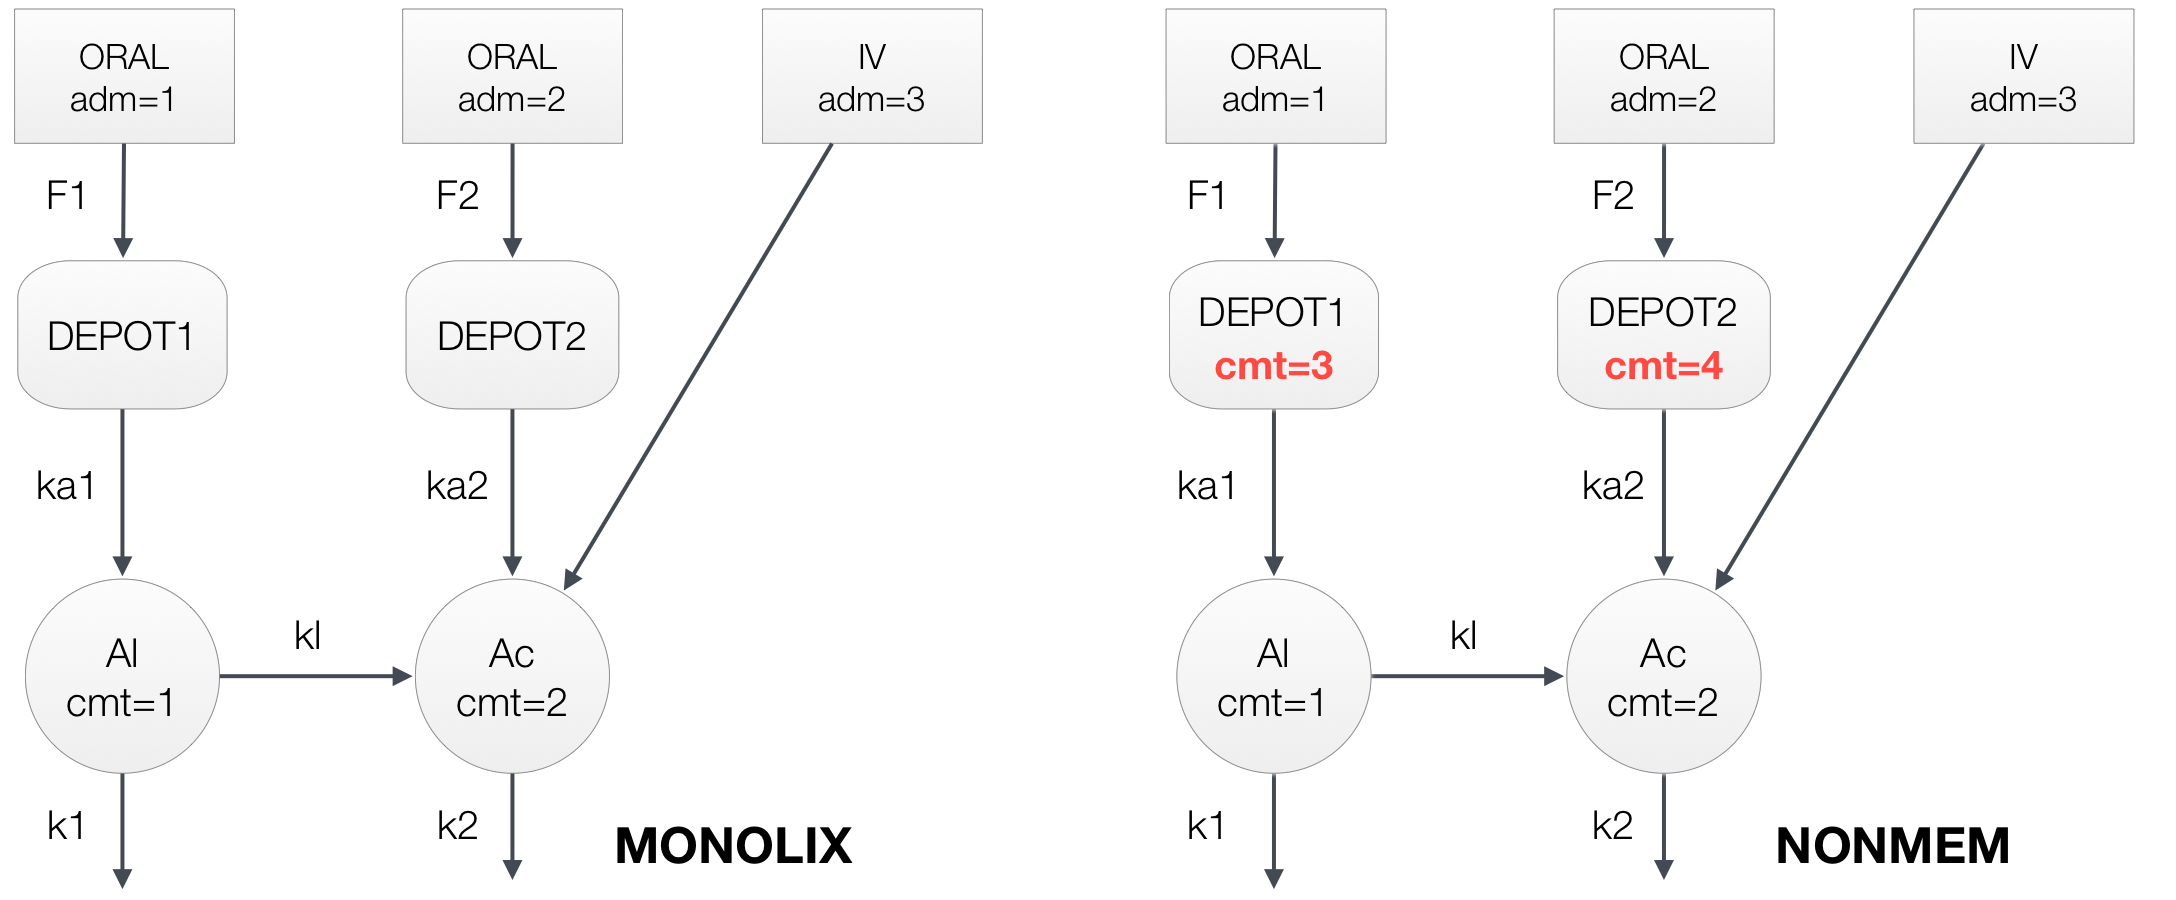
\includegraphics[width=120mm]{pics/ComplexModel3}
%\caption{Two model interpretations for a model with more then one administration 
%from which at least one is of oral type, dependent on the target tool. 
%While MONOLIX (left) doesn't assign a number to the depot compartment, 
%NONMEM (right) does. The difference is inter-connected with the format of the 
%dataset compatible with each model version, see Table \ref{tab:datasetComparison}.}
%\label{fig:ComplexModel3A}
%\end{figure}
%
%
%\begin{table}[ht!]
%\footnotesize
%\parbox{.5\linewidth}{
%\centering
%\begin{tabular}{ccccc}
%  \hline
%     \multicolumn{5}{c}{\textbf{MONOLIX}} \\
%  \hline
%ID	& TIME  & AMT	 & \textbf{ADM} &	Y \\
%  \hline
%1	& 0	    & 2.24	& \textbf{2}	& . \\
%1	& 1	    & .	& .		 	& 142 \\
%1	& 2	    & .	& .	 		& 54.9 \\
%1	& 3	    & .	& .			& 25.9 \\
%1	& 4	    & .	& .			& 17.5 \\
%1	& 6	    & 7	& \textbf{1}	& . \\
%1	& 7	    & .	& .			& 192 \\
%1	& 8	    & .	& .			& 141 \\
%1	& 9	    & .	& .			& 189 \\
%2	& 0	    & 2.73	& \textbf{2}	& . \\
%2	& 1	    & . 	& .			& 176 \\
%...     &  ...     &  ...     & ...  			& ...\\
%\end{tabular}
%}
%\hfill
%\parbox{.5\linewidth}{
%\centering
%\begin{tabular}{ccccc}
%  \hline
%   \multicolumn{5}{c}{\textbf{NONMEM}} \\
%  \hline
%ID	& TIME  & AMT	 & \textbf{\textcolor{red}{CMT}} &	Y \\
%  \hline
%1	& 0	    & 2.24	& \textbf{\textcolor{red}{1}}	& . \\
%1	& 1	    & .	& .		 	& 142 \\
%1	& 2	    & .	& .	 		& 54.9 \\
%1	& 3	    & .	& .			& 25.9 \\
%1	& 4	    & .	& .			& 17.5 \\
%1	& 6	    & 7	& \textbf{\textcolor{red}{2}}	& . \\
%1	& 7	    & .	& .			& 192 \\
%1	& 8	    & .	& .			& 141 \\
%1	& 9	    & .	& .			& 189 \\
%2	& 0	    & 2.73	& \textbf{\textcolor{red}{1}}	& . \\
%2	& 1	    & . 	& .	 		& 176 \\
%...     &  ...     &  ...     & ...  			& ...\\
%\end{tabular}
%}
%\caption{Comparison of NONMEM and MONOLIX datasets for the model shown 
%in Figure \ref{fig:ComplexModel3A}. NONMEM requires additionally a CMT column in 
%the dataset, whereas MONOLIX doesn't and uses instead administration type number
%stored in the ADM column.}
%\label{tab:datasetComparison}
%\end{table}


%\newpage
\subsubsection{Datasets mapping}
We will discuss now briefly the mapping between macros and the MONOLIX dataset, 
i.e. the mapping between \xatt{adm/type} attributes in the PK macros and the 
administration type as stored in the ADM column,
\begin{itemize}
\item 
\xelem{TargetMapping} element with the \xatt{blkIdRef} attribute, the latter one because 
in PharmML multiple structural models are allowed, so we have to specify which model is 
holding the target compartment definition
\item
\xelem{Map} element with
\begin{itemize}
\item 
\xatt{dataSymbol} -- attribute denoting the target symbol as encoded in a dataset and
\item 
new attribute \xatt{admNumber} -- to identify the target symbol in the model.
\end{itemize}
\end{itemize}

%\xatt{modelSymbol}/\xatt{cmtNumber}/

The use of these new elements is explained in the Table \ref{tab:mappingNONMEMAndMacros}. 
%(Left) the mapping if MONOLIX dataset is used, {right} for the NONMEM dat set.
\begin{table}[ht!]
\setlength{\tabcolsep}{5pt}
\centering
\begin{tabular}{l}
  \hline
  \hline
MONOLIX datasets mapping \\ %  	& NONMEM datasets mapping \\
  \hline
\lstset{language=XML}
\begin{lstlisting}
<ExternalDataSet toolName="Monolix" oid="MLXoid">
    <!-- omitted details -->
    <ColumnMapping>
        <ds:ColumnRef columnIdRef="ADM"/>
        <ds:TargetMapping blkIdRef="sm3">
            <ds:Map dataSymbol="1" admNumber="1"/>
            <ds:Map dataSymbol="2" admNumber="2"/>
            <ds:Map dataSymbol="3" admNumber="3"/>
        </ds:TargetMapping>
    </ColumnMapping>
    <!-- omitted ColumnMappings and Definition of dataset with ID,TIME,AMT,ADM  -->
\end{lstlisting}
%&
%\lstset{language=XML}
%\begin{lstlisting}
%<NONMEMdataSet oid="NMoid">
%    <!-- omitted details -->
%    
%    <ColumnMapping>
%        <ds:ColumnRef columnIdRef="CMT"/>
%        <ds:TargetMapping blkIdRef="sm3">
%            <ds:Map dataSymbol="2" cmtNumber="2"/>
%            <ds:Map dataSymbol="3" cmtNumber="3"/>
%            <ds:Map dataSymbol="4" cmtNumber="4"/>
%        </ds:TargetMapping>
%    </ColumnMapping>
%    
%    <!-- omitted Definition of dataset  
%    	columns such as ID,TIME,AMT,CMT  -->
%\end{lstlisting}
%\\
%& OR \\
%&
%\lstset{language=XML}
%\begin{lstlisting}
%<NONMEMdataSet oid="NMoid">
%    <!-- omitted details -->
%    
%    <ColumnMapping>
%        <ds:ColumnRef columnIdRef="CMT"/>
%        <ds:TargetMapping blkIdRef="sm3">
%            <ds:Map dataSymbol="2" modelSymbol="Ac"/>
%            <ds:Map dataSymbol="3" modelSymbol="Depot1"/>
%            <ds:Map dataSymbol="4" modelSymbol="Depot2"/>
%        </ds:TargetMapping>
%    </ColumnMapping>
%    
%    <!-- omitted Definition of dataset  
%    	columns such as ID,TIME,AMT,CMT  -->
%\end{lstlisting}
\\
    \hline
\end{tabular}
\caption{Mappings of MONOLIX type datasets and PK macros.}
\label{tab:mappingNONMEMAndMacros}
\end{table}



%\newpage
%%%%%%%%%%%%%%%%%%%%%%%%%%%%%%%%%%%%%%%%%%%%%%%%%%%%%%%%%
\subsection{Linking macros and \xelem{TrialDesign}}
\label{subsec:LinkingMacrosTrialDesign}
\xelem{TrialDesign} section provides an alternative to encode design and to store 
data records (observations, dosing and covariates) in a tool-independent manner. 
The \xelem{IndividualDosing} element is the place where relevant dosing data can 
be encoded inline or be referred to from an external datafile. The actual mapping 
is defined within the \xelem{Activity} tag.

A minor extension in the \xelem{TrialDesign} is necessary to link the administrations coded
in \xelem{Activity} elements  to the targets in the PK macros and identified using the 
\xatt{adm} attribute, i.e.
\begin{itemize}
\item
new value \textit{administrationType} is added to the \xatt{inputTarget} attribute.
\end{itemize}
Otherwise, elements defined in the last section will be reused. The Table 
\ref{tab:mappingTrialDesignAndMacros} shows the implementations within the 
\xelem{TrialDesign} element in cases when (left) a PK model is expressed using 
algebraic equation with dose parameter, D, and (right) when using PK macros.
\begin{table}[ht!]
\setlength{\tabcolsep}{5pt}
\centering
\begin{tabular}{ll}
  \hline
  \hline
Using dose \xatt{parameter}, D, and algebraic & Using value \emph{administrationType} for \xatt{inputTarget}  \\
equation for PK model, e.g. $C(t)=f(D,V,k,...)$ 	& and \xelem{TargetMapping}/\xelem{Map} elements   \\
(available in PharmML since version 0.2.1)	& 	\\
  \hline
\lstset{language=XML}
\begin{lstlisting}
<Activity oid="actBolusD">
    <Bolus>
        <DoseAmount inputTarget="parameter">
            <ct:SymbRef blkIdRef="sm3" symbIdRef="D"/>
            <ct:Assign>
                <ct:Real>10</ct:Real>
            </ct:Assign>
        </DoseAmount>
        <DosingTimes>
            <!-- e.g. 10 -->
        </DosingTimes>
    </Bolus>
</Activity>
\end{lstlisting}
&
\lstset{language=XML}
\begin{lstlisting}
<Activity oid="actBolusMacro">
    <Bolus>
        <DoseAmount inputTarget="admType">
            <ds:TargetMapping blkIdRef="sm3">
                <ds:Map admNumber="2"/>
            </ds:TargetMapping>
            <ct:Assign>
                <ct:Real>10</ct:Real>
            </ct:Assign>
        </DoseAmount>
        <!-- omitted DosingTimes -->
    </Bolus>
</Activity>
\end{lstlisting}
\\
    \hline
\end{tabular}
\caption{Comparison of the link between administration definitions and structural model. 
(left) PK model expressed using algebraic equations
 with dose parameter, $D$, and when using the PK macros (right).}
\label{tab:mappingTrialDesignAndMacros}
\end{table}


%{\color{red} \scshape{NEW}}
%\newpage
%%%%%%%%%%%%%%%%%%%%%%%%%%%%%%%%%%%%%%%%%%%%%%%%%%%%%%%%%
\subsection{Connection between macros and the model}
\label{subsec:macroOutputLink}
The possible outputs of PK macros are amounts, e.g. $Ac$, and concentrations, e.g. $C$. 
A PK model defined by a system of macros will often be connected to a subsequent PD 
model, which expects the concentration, $C$, as one of the inputs. Another option is that the output
of the PK macros will be mapped directly to the data in the \xelem{ObservationModel}. 

For the \emph{compartment} macro in question, there are two possibilities, either
\begin{itemize}
\item
the concentration is defined in the macro
\lstset{language=NONMEMdataSet}
\begin{lstlisting}
		compartment(cmt=1,concentration=C, volume=V)
\end{lstlisting}
in which case no output has to be defined explicitly, or
\item
the alternative form of this macro is used
\lstset{language=NONMEMdataSet}
\begin{lstlisting}
		compartment(cmt=1,amount=Ac, volume=V)
\end{lstlisting}
and because eventually the concentration is required, a subsequent assignment for $C$ must be provided in MLXTRAN
in the \emph{EQUATION} block, i.e. $C = Ac/V$
\end{itemize}
In PharmML, these two cases have to be treated accordingly. 
\begin{itemize}
\item
In the first case only the concentration variable, $C$, needs to be defined
\lstset{language=XML}
\begin{lstlisting}
        <StructuralModel blkId="sm1">
            <ct:Variable symbolType="real" symbId="C"/>
            <PKmacros>
                    <!-- omitted details of the macro compartment(cmt=1,concentration=C, volume=V) -->
\end{lstlisting}
\item
in the second case, both the amount variable, $Ac$, and concentration variable, $C$, 
with the $C=Ac/V$ assignment needs to be defined
\lstset{language=XML}
\begin{lstlisting}
        <StructuralModel blkId="sm1">
            <ct:Variable symbolType="real" symbId="Ac"/>
            <ct:Variable symbolType="real" symbId="Cc">
                <ct:Assign>
                    <math:Equation>
                        <math:Binop op="divide">
                            <ct:SymbRef symbIdRef="Ac"/>
                            <ct:SymbRef blkIdRef="pm1" symbIdRef="V"/>
                        </math:Binop>
                    </math:Equation>
                </ct:Assign>
            </ct:Variable>
            
            <PKmacros>
                <Compartment>
                    <!-- omitted details of the macro compartment(cmt=1,amount=Ac, volume=V) -->
\end{lstlisting}
\end{itemize}
If a model using the PK macros is defined properly, following the principles described above, 
both options make sure that the connection to a subsequent model or the \xelem{ObservationModel} 
can be established.



%%%%%%%%%%%%%%%%%%%%%%%%%%%%%%%%%%%%%%%%%%%%%%%%%%%%%%%%%%%%%%%%%%%%%%
\section{PREDPP models and PK macros}
\label{subsec:PREDPPinMACROS}
This section describes PREDPP library models as encoded in routines ADVAN1-4 and 10-12 
and their PK macros implementation. 
As explained in Section \ref{subsec:LinkingMacrosDatasets} there are differences between 
NONMEM and MONOLIX and their datasets one has to consider when dealing with PK macros.
They manifest themselves also in that way how the transfer rate constants are numbered/named. 
Models with more then two compartments and with 1st order input (using \emph{DEPOT} 
compartment) will have different transfer rate symbols, e.g.:
\begin{itemize}
\item
ADVAN 4
\begin{table}[ht]
\centering
\small
\renewcommand{\arraystretch}{1.1}% 
\begin{tabular}{lcc}
  \hline
  \hline
				 	& PREDPP routines 	& PK macros \\
  \hline
transfer rate constants 	& k23, k32 		& k12, k21 \\
\hline
\end{tabular}
\end{table}
\item
ADVAN 12
\begin{table}[h!]
\centering
\small
\renewcommand{\arraystretch}{1.1}% 
\begin{tabular}{lcc}
  \hline
  \hline
				 	& PREDPP routines 	& PK macros \\
  \hline
transfer rate constants 	& k23, k32 		& k12, k21  \\
					& k24, k42 		& k13, k31  \\
\hline
\end{tabular}
\end{table}
\end{itemize}
Models described in this section use the MLXTRAN numbering convention in order to comply
with the PK macros notation.

To allow for a lossless translation between PREDPP coded models and PK macros one needs
to establish well defined translation rules. To achieve this goal and provide help to other 
translation/converter teams one needs to analyse the predefined PREDPP routines ADVAN1-4 \& 10-12
and more specifically to
\begin{enumerate}
\item
understand what they mean
\item
dissect the routines into elementary components and finally 
\item
find equivalent formulation for each such element in the PK macro speak.
\end{enumerate}
The above steps are illustrated in Table \ref{tab:ADVAN_translation} in an abbreviated form. 
In the column \emph{Interpretation} first two steps are implemented, 
the last column provides the according PK macro formulation.

\begin{center}
\begin{longtable}{lll}
  \hline
  \hline
ADVAN routine & Interpretation & MLXTRAN macro \\
\& default TRANS1 &		& \\
%ADVAN\_X & Interpretation & Elements & MLXTRAN macro \\
%(w. TRANS1)		&			 &		    &	\\
\hline
\multicolumn{3}{c}{one compartment}  \\[.1ex]
\hline
%1-comp, IV input
\lstset{language=NONMEMdataSet}
\begin{lstlisting}
ADVAN1
compartment
\end{lstlisting}
&
\lstset{language=Elements}
\begin{lstlisting}
- 1 compartment

- iv bolus administration

- linear elimination
\end{lstlisting}
& 
\lstset{language=MLXTRANcode}
\begin{lstlisting}
compartment(cmt=1, amount=Ac, volume=V)

iv(adm=1, cmt=1)

elimination(cmt=1, k)
\end{lstlisting} 

\\
& 
\\
\hdashline


%1-comp, 1st order input
\lstset{language=NONMEMdataSet}
\begin{lstlisting}
ADVAN2
\end{lstlisting}
&
\lstset{language=Elements}
\begin{lstlisting}
- 1 compartment

- oral administration, 1st order absorption

- linear elimination
\end{lstlisting}
%&
%
&
\lstset{language=MLXTRANcode}
\begin{lstlisting}
compartment(cmt=1, amount=Ac, volume=V)

oral(adm=1, cmt=1, ka)

elimination(cmt=1, k)
\end{lstlisting}

\\
& 
\\
\hdashline

%1-comp, IV input 
%with saturable elimination
\lstset{language=NONMEMdataSet}
\begin{lstlisting}
ADVAN10
\end{lstlisting}
&
\lstset{language=Elements}
\begin{lstlisting}
- 1 compartment

- iv bolus administration

- saturable elimination
\end{lstlisting}
%&
%
&
\lstset{language=MLXTRANcode}
\begin{lstlisting}
compartment(cmt=1, amount=Ac, volume=V)

iv(adm=1, cmt=1)

elimination(cmt=1, Km, Vm)
\end{lstlisting}

\\
\hline
\multicolumn{3}{c}{two compartments}  \\[.1ex]

  \hline

%2-comp, IV input
\lstset{language=NONMEMdataSet}
\begin{lstlisting}
ADVAN3 
\end{lstlisting}
&
\lstset{language=Elements}
\begin{lstlisting}
- 2 compartments 
one central (1) & one peripheral with
linear transfer rates

- iv bolus administration (into 1)

- linear elimination (from 1)
\end{lstlisting}
%&
%
&
\lstset{language=MLXTRANcode}
\begin{lstlisting}
compartment(cmt=1, amount=Ac, volume=V)
peripheral(k12, k21, amount=Ap)


iv(adm=1, cmt=1)

elimination(cmt=1, k)
\end{lstlisting}

\\
& 
\\
\hdashline


%2-comp, 1st order input 
\lstset{language=NONMEMdataSet}
\begin{lstlisting}
ADVAN4 
\end{lstlisting}
&
\lstset{language=Elements}
\begin{lstlisting}
- 2 compartments 
one central (1) & one peripheral with
linear transfer rates

- oral administration, 1st order absorption 
(into 1)

- linear elimination (from 1)
\end{lstlisting}
%&
%
&
\lstset{language=MLXTRANcode}
\begin{lstlisting}
compartment(cmt=1, amount=Ac, volume=V)
peripheral(k12, k21, amount=Ap)


oral(adm=1, cmt=1, ka)

elimination(cmt=1, k)
\end{lstlisting}

\\
\hline
\multicolumn{3}{c}{three compartments}  \\[.1ex]
  \hline
  
%3-comp, IV input 
\lstset{language=NONMEMdataSet}
\begin{lstlisting}
ADVAN11
\end{lstlisting}
&
\lstset{language=Elements}
\begin{lstlisting}
- 3 compartments 
one central (1) & two peripheral with
linear transfer rates

- iv bolus administration (into 1)

- linear elimination (from 1)
\end{lstlisting}
%&
%
&
\lstset{language=MLXTRANcode}
\begin{lstlisting}
compartment(cmt=1, amount=Ac, volume=V)
peripheral(k12, k21, amount=Ap1)
peripheral(k13, k31, amount=Ap2)

iv(adm=1, cmt=1)

elimination(cmt=1, k)
\end{lstlisting}

\\
& 
\\
\hdashline

%3-comp, 1st order input 
\lstset{language=NONMEMdataSet}
\begin{lstlisting}
ADVAN12
\end{lstlisting}
&
\lstset{language=Elements}
\begin{lstlisting}
- 3 compartments 
one central (1) & two peripheral with
linear transfer rates

- oral administration, 1st order absorption 
(into 1)

- linear elimination (from 1)
\end{lstlisting}
%&
%
&
\lstset{language=MLXTRANcode}
\begin{lstlisting}
compartment(cmt=1, amount=Ac, volume=V)
peripheral(k12, k21, amount=Ap1)
peripheral(k13, k31, amount=Ap2)

oral(adm=1, cmt=1, ka)

elimination(cmt=1, k)
\end{lstlisting}
    \\ [+1ex]
      \hline
      \\
\caption{Interpretation and translation of PREDPP models using ADVAN1-4 \& 10-12 routines, 
with default TRANS1 parameterization, into PK macros.}
\label{tab:ADVAN_translation}
\end{longtable}
\end{center}

\begin{figure}[htbp!]
\centering
 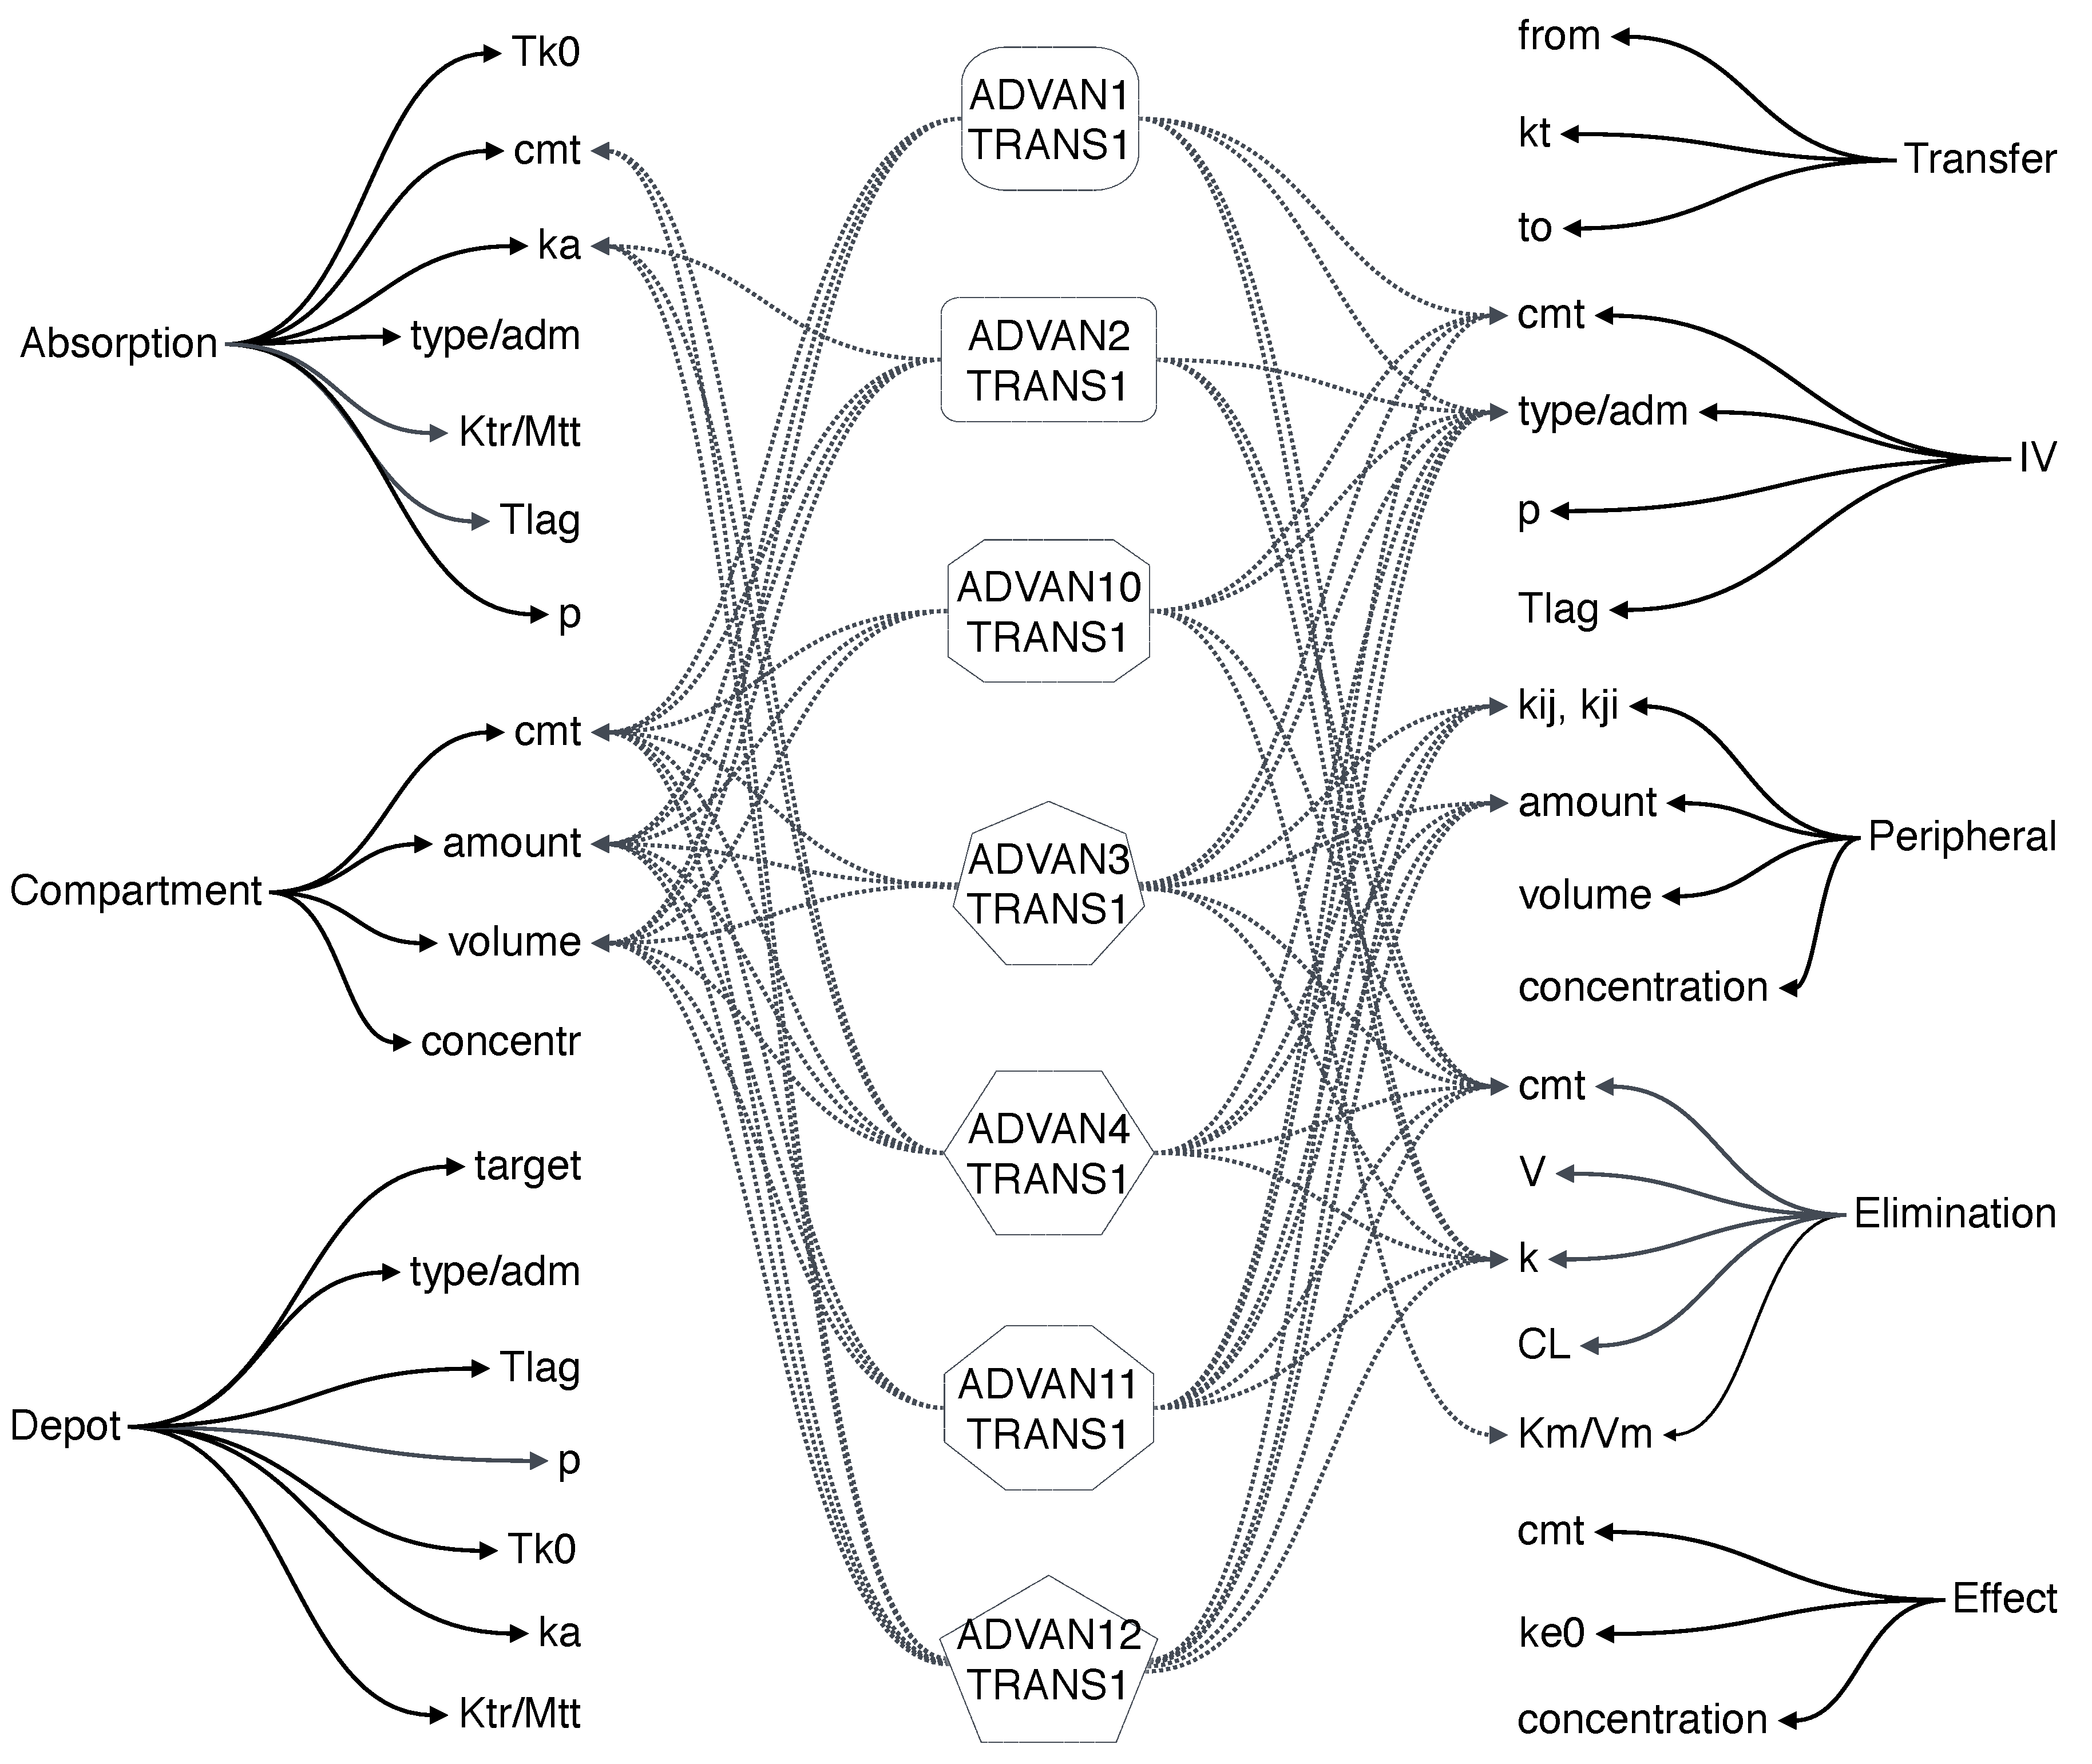
\includegraphics[width=170mm]{pics/AdvanMacrosMaster.pdf}
\caption{The overview of the ADVAN models, with their default parameterisation TRANS1, 
and their connection to PK macros based on the analysis in Table \ref{tab:ADVAN_translation}. 
Each ADVAN model can be uniquely mapped to macros and their attributes. For more 
details see next section with examples.}
\label{fig:AdvanMacrosMaster}
\end{figure}


%%%%%%%%%%%%%%%%%%%%%%%%%%%%%%%%%%%%%%%%%%%%%%%%%%%%%%%%%%%%%%%%%%%%%%
\section{Examples}
\label{subsec:PREDPPinMACROSExamples}

We will conclude this section with two examples of PREDPP coded models 
and show their implementation in PK macros in PharmML, which will
illustrate number of aspects described in the previous sections such as 
interpretation of the models, their translation and the associated dataset 
conversion.

%%%%%%%%%%%%%%%%%%%%%%%%%%%%%%%%%%%%%%%%%%%%%%%%%%%%%%%%%%%%%%%%%%%%%%
\subsection{ADVAN4, TRANS1 -- 2-comp 1st order input}
ODE formulation:
\begin{align}
\frac{dAd}{dt} &= -ka \times Ad \nonumber \\
\frac{dAc}{dt} &= ka \times Ad - k_{12} \times Ac + k_{21} \times Ap - k \times Ac  \nonumber \\
\frac{dAp}{dt} &= k_{12} \times Ac - k_{21} \times Ap  \nonumber
\end{align}

\begin{figure}[htbp!]
\centering
 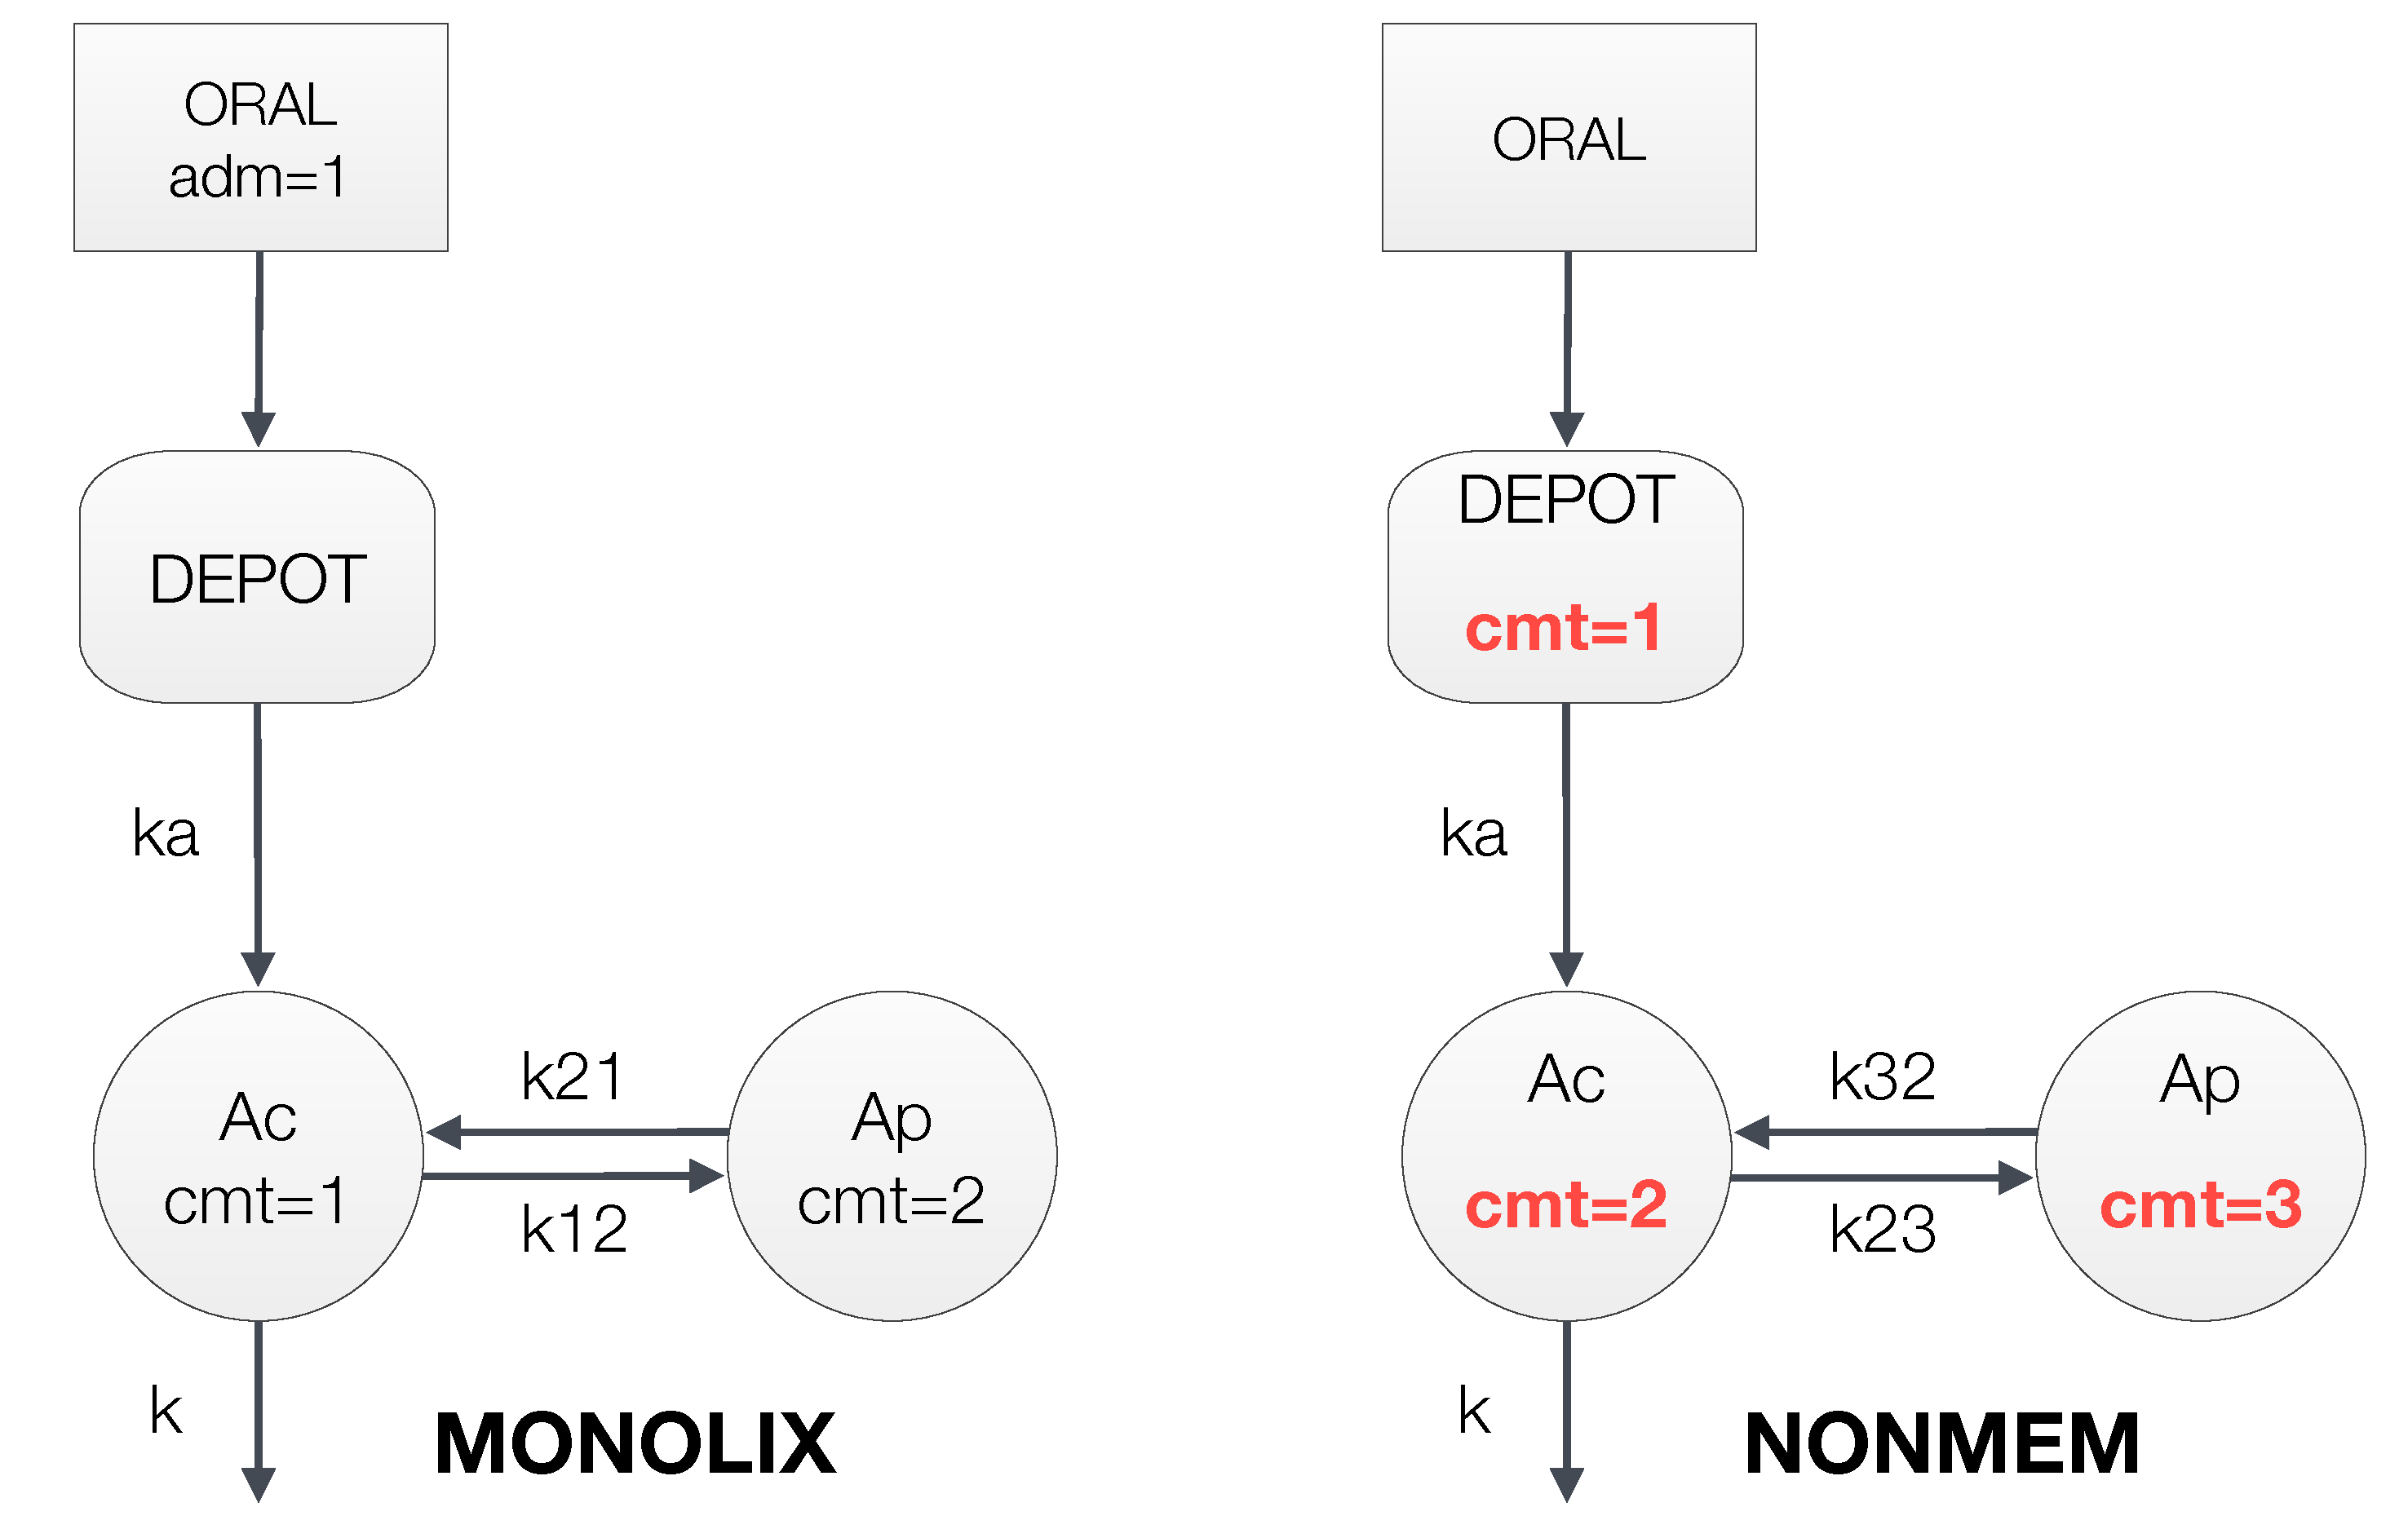
\includegraphics[width=110mm]{pics/Advan4.pdf}
\caption{ADVAN4 model, with compartment numbering dependent on the target tool. 
Note, that not only the compartment numbers are different in NONMEM coded model, 
the rate constants names are different as well.}
\label{fig:Advan4}
\end{figure}


\begin{table}[ht!]
\footnotesize
\parbox{.5\linewidth}{
\centering
\begin{tabular}{ccccc}
  \hline
   \multicolumn{5}{c}{\textbf{MONOLIX}} \\
  \hline
ID & TIME & AMT & \textbf{ADM} & Y \\
  \hline
1  & 0        & 10   & \textbf{1} & .       \\
1  & 2        & .      & . & 5        \\
... &  ...      &  ...   &  ...&  ...     \\
\end{tabular}
}
\hfill
\parbox{.5\linewidth}{
\centering
\begin{tabular}{ccccc}
  \hline
   \multicolumn{5}{c}{\textbf{NONMEM}} \\
  \hline
ID & TIME & AMT & \textbf{\textcolor{red}{CMT}} & DV \\
  \hline
1  & 0        & 10   & \textbf{\textcolor{red}{1}}   & .    \\
1  & 2        & .      & 2    & 5   \\
... &  ...      &  ...   &  ... & ...  \\
\end{tabular}
}
\caption{MONOLIX and NONMEM datasets for the ADVAN4 model.}
\end{table}

\begin{table}[h!]
\setlength{\tabcolsep}{15pt}
\begin{center}
%\begin{tabular*}{.95\textwidth}{@{\extracolsep{\fill} } ll}
\begin{tabular}{l}
  \hline \hline
PK macro  \\[-.25ex]
  \hline
\lstset{language=NONMEMdataSet}
\begin{lstlisting}
compartment(cmt=1, amount=Ac, volume=V)
peripheral(k12, k21, amount=Ap)
oral(adm=1, cmt=1, ka)
elimination(cmt=1, k)
\end{lstlisting}
%&
%\lstset{language=NONMEMdataSet}
%\begin{lstlisting}
%input = {ka, V, k, k12, k21}
%PK:
%compartment(cmt=1, amount=Ac, volume=V)
%[*compartment(cmt=3, amount=Depot)*]
%peripheral(k12, k21, amount=Ap)
%oral(adm=1, [*fromCmt=3,*] cmt=1, ka)
%elimination(cmt=1, k)
%\end{lstlisting} 
\\
  \hline
\end{tabular}
\caption{PK macros  for the ADVAN4 model, as shown in Figure \ref{fig:Advan4} (left).}
\label{tab:advan4Table}
\end{center}
\end{table}

PharmML code:
\lstset{language=XML}
\begin{lstlisting}
        <StructuralModel blkId="sm4">
            <ct:Variable symbolType="real" symbId="Ac"/>
            <ct:Variable symbolType="real" symbId="Ap"/>
            <ct:Variable symbolType="real" symbId="Cc">
                <ct:Assign>
                    <math:Equation>
                        <math:Binop op="divide">
                            <ct:SymbRef symbIdRef="Ac"/>
                            <ct:SymbRef blkIdRef="pm1" symbIdRef="V"/>
                        </math:Binop>
                    </math:Equation>
                </ct:Assign>
            </ct:Variable>
            <PKmacros>
                <Compartment>
                    <Value argument="cmt">
                        <ct:Int>1</ct:Int>
                    </Value>
                    <Value argument="amount">
                        <ct:SymbRef symbIdRef="Ac"/>
                    </Value>
                    <Value argument="volume">
                        <ct:SymbRef blkIdRef="pm1" symbIdRef="V"/>
                    </Value>
                </Compartment>
                <Peripheral>
                    <Value>
                        <ct:SymbRef blkIdRef="pm1" symbIdRef="k12"/>
                    </Value>
                    <Value>
                        <ct:SymbRef blkIdRef="pm1" symbIdRef="k21"/>
                    </Value>
                    <Value argument="amount">
                        <ct:SymbRef symbIdRef="Ap"/>
                    </Value>
                </Peripheral>
                <Oral>
                    <Value argument="adm">
                        <ct:Int>1</ct:Int>
                    </Value>
                    <Value argument="cmt">
                        <ct:Int>1</ct:Int>
                    </Value>
                    <Value>
                        <ct:SymbRef blkIdRef="pm1" symbIdRef="ka"/>
                    </Value>
                </Oral>
                <Elimination>
                    <Value argument="cmt">
                        <ct:Int>1</ct:Int>
                    </Value>
                    <Value>
                        <ct:SymbRef blkIdRef="pm1" symbIdRef="k"/>
                    </Value>
                </Elimination>
            </PKmacros>
        </StructuralModel>
\end{lstlisting}


%%%%%%%%%%%%%%%%%%%%%%%%%%%%%%%%%%%%%%%%%%%%%%%%%%%%%%%%%%%%%%%%%%%%%%
\subsection{ADVAN12, TRANS1 -- 3-comp 1st order input}
\label{subsubsec:ADVAN12}
ODE formulation:
\begin{align}
\frac{dAd}{dt} & =  -ka \times Ad \nonumber \\
\frac{dAc}{dt} & = ka \times Ad - k_{12} \times Ac + k_{21} \times Ap1 - k_{13} \times Ac \nonumber \\
			& + k_{31} \times Ap2 - k \times Ac  \nonumber \\
\frac{dAp1}{dt} & =  k_{12} \times Ac - k_{21} \times Ap1  \nonumber \\
\frac{dAp2}{dt} & =  k_{13} \times Ac - k_{31} \times Ap2  \nonumber
\end{align}

\begin{figure}[htbp!]
\centering
 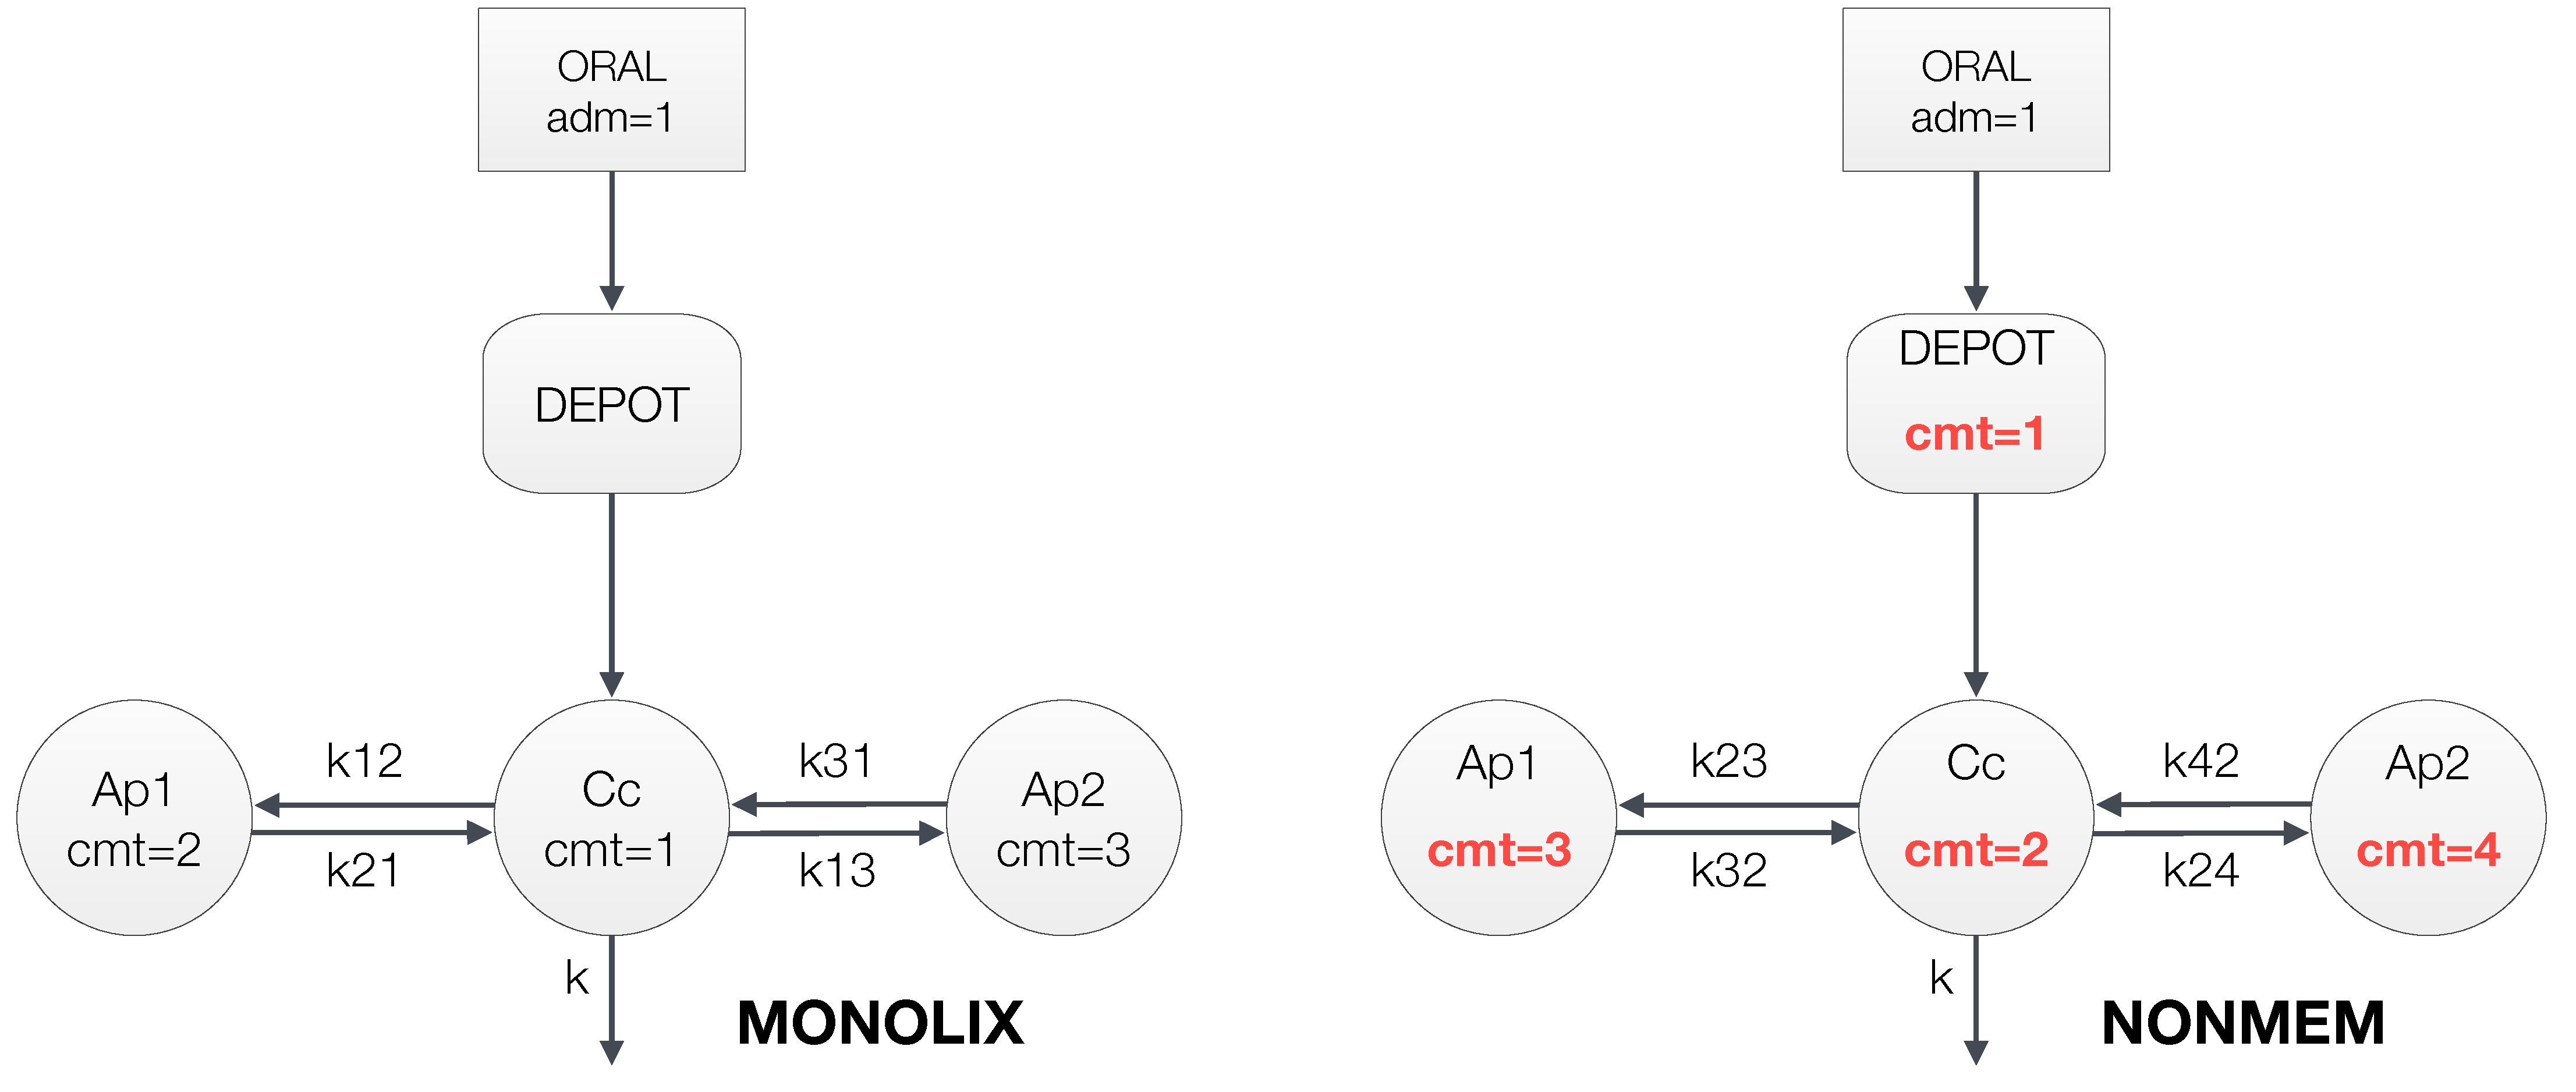
\includegraphics[width=160mm]{pics/Advan12.pdf}
\caption{ADVAN12 model, with compartment numbering dependent on the target tool. 
Note, that not only the compartment numbers are different in NONMEM coded model, 
the rate constants names are different as well.}
\label{fig:Advan12}
\end{figure}


\begin{table}[ht!]
\footnotesize
\parbox{.5\linewidth}{
\centering
\begin{tabular}{ccccc}
  \hline
   \multicolumn{5}{c}{\textbf{MONOLIX}} \\
  \hline
ID & TIME & AMT & \textbf{ADM} & Y \\
  \hline
1  & 0        & 10   & \textbf{1} & .       \\
1  & 2        & .      & . 	& 5        \\
... &  ...      &  ...   &  ...  &  ...     \\
\end{tabular}
}
\hfill
\parbox{.5\linewidth}{
\centering
\begin{tabular}{ccccc}
  \hline
   \multicolumn{5}{c}{\textbf{NONMEM}} \\
  \hline
ID & TIME & AMT & \textbf{\textcolor{red}{CMT}} & DV \\
  \hline
1  & 0        & 10   & \textbf{\textcolor{red}{1}}   & .    \\
1  & 2        & .      & 2    & 5   \\
... &  ...      &  ...   &  ... & ...  \\
\end{tabular}
}
\caption{MONOLIX and NONMEM datasets for the ADVAN12 model.}
\end{table}


\begin{table}[h!]
\setlength{\tabcolsep}{15pt}
\begin{center}
%\begin{tabular*}{.95\textwidth}{@{\extracolsep{\fill} } ll}
\begin{tabular}{l}
  \hline \hline
PK macro \\[-.25ex]
  \hline
\lstset{language=NONMEMdataSet}
\begin{lstlisting}
compartment(cmt=1, amount=Ac, volume=V)
peripheral(k12, k21, amount=Ap1)
peripheral(k13, k31, amount=Ap2)
oral(adm=1, cmt=1, ka)
elimination(cmt=1, k)
\end{lstlisting}
\\
  \hline
\end{tabular}
\caption{PK macros  for the ADVAN12 model, as shown in Figure \ref{fig:Advan12} (left).}
\label{tab:advan12Table}
\end{center}
\end{table}


PharmML code:
\lstset{language=XML}
\begin{lstlisting}
        <StructuralModel blkId="sm12">
            <ct:Variable symbolType="real" symbId="Ac"/>
            <ct:Variable symbolType="real" symbId="Ap1"/>
            <ct:Variable symbolType="real" symbId="Ap2"/>
            <ct:Variable symbolType="real" symbId="Cc">
                <ct:Assign>
                    <math:Equation>
                        <math:Binop op="divide">
                            <ct:SymbRef symbIdRef="Ac"/>
                            <ct:SymbRef blkIdRef="pm1" symbIdRef="V"/>
                        </math:Binop>
                    </math:Equation>
                </ct:Assign>
            </ct:Variable>
            
            <PKmacros>
                <Compartment>
                    <Value argument="cmt">
                        <ct:Int>1</ct:Int>
                    </Value>
                    <Value argument="amount">
                        <ct:SymbRef symbIdRef="Ac"/>
                    </Value>
                    <Value argument="volume">
                        <ct:SymbRef blkIdRef="pm1" symbIdRef="V"/>
                    </Value>
                </Compartment>
                <Peripheral>
                    <Value>
                        <ct:SymbRef blkIdRef="pm1" symbIdRef="k12"/>
                    </Value>
                    <Value>
                        <ct:SymbRef blkIdRef="pm1" symbIdRef="k21"/>
                    </Value>
                    <Value argument="amount">
                        <ct:SymbRef symbIdRef="Ap1"/>
                    </Value>
                </Peripheral>
                <Peripheral>
                    <Value>
                        <ct:SymbRef blkIdRef="pm1" symbIdRef="k13"/>
                    </Value>
                    <Value>
                        <ct:SymbRef blkIdRef="pm1" symbIdRef="k31"/>
                    </Value>
                    <Value argument="amount">
                        <ct:SymbRef symbIdRef="Ap2"/>
                    </Value>
                </Peripheral>
                <Oral>
                    <Value argument="adm">
                        <ct:Int>1</ct:Int>
                    </Value>
                    <Value argument="cmt">
                        <ct:Int>1</ct:Int>
                    </Value>
                    <Value>
                        <ct:SymbRef blkIdRef="pm1" symbIdRef="ka"/>
                    </Value>
                </Oral>
                <Elimination>
                    <Value argument="cmt">
                        <ct:Int>1</ct:Int>
                    </Value>
                    <Value>
                        <ct:SymbRef blkIdRef="pm1" symbIdRef="k"/>
                    </Value>
                </Elimination>
            </PKmacros>
        </StructuralModel>
\end{lstlisting}
\subparagraph{Note} A detailed description of all remaining predefined PREDPP models 
(ADVAN 1-3, 10, 11), alternative parameterizations other then the default TRANS1 as well 
aa more complex examples of macro implementation can be found in a technical report 
\cite{PKmacros:2015a} on PharmML related websites \url{http://ddmore.eu/pharmml} or 
\url{http://pharmml.org}.


